\documentclass[12pt,openany]{report}
\usepackage[utf8]{inputenc}
\usepackage[T1]{fontenc}
\usepackage[spanish, es-noshorthands]{babel}
\usepackage{graphicx}
\usepackage{float}
\usepackage{enumitem}
\usepackage{geometry}
\usepackage{xcolor}
\usepackage{titlesec}
\usepackage{hyperref}
\usepackage{colortbl}
\usepackage{longtable}
\usepackage{multirow}
\usepackage{array}
\usepackage{tcolorbox}                       % Cajas con color
\usepackage{forest}
\usepackage{pifont}      % para \ding{51} (checkmark) y \ding{55} (cross)
\usepackage{verbatim}
% Definir un estilo de árbol para el EDT
\forestset{
  edt/.style={
    for tree={
      draw,                % borde alrededor de cada nodo
      rounded corners,
      align=center,
      text width=2.8cm,
      font=\small,
      parent anchor=south,
      child anchor=north,
      edge={->, thick},    % flecha de conexión
      l sep=1cm,           % separación vertical entre niveles
      s sep=1cm,           % separación horizontal entre nodos hermanos
      tier/.option=level   % alinea nodos del mismo nivel
    }
  }
}
\geometry{a4paper, margin=2.5cm}



% Configuración de títulos de capítulo
% Mostrar "Capítulo N: Título" en el encabezado del capítulo
\titleformat{\chapter}[hang]{\huge\bfseries}{Capítulo \ \thechapter:}{1em}{}
\titlespacing*{\chapter}{0pt}{-20pt}{20pt}

% Configuración de títulos de sección
\titleformat{\section}{\Large\bfseries}{}{0em}{}
\titleformat{\subsection}{\large\bfseries}{}{0em}{}
\titleformat{\subsubsection}{\normalsize\bfseries\itshape}{}{0em}{}

\hypersetup{
    colorlinks=true,
    linkcolor=black,
    urlcolor=blue,
}



\begin{document}
\raggedbottom
% ==== PORTADA ====
%PORTADA
\begin{titlepage}
    \begin{center}
        \vspace*{-1in}

        \begin{Huge}
            \textbf{Proyecto Final\\}
        \end{Huge}
        \vspace*{0.1in}
        \begin{huge}
            Análisis de los hábitos de escucha en Spotify\\
        \end{huge}

        \vspace*{0.4in}
        \begin{tcolorbox}[colback=white]
            \begin{Huge}
                \begin{center}
                    \textbf{Técnicas de Ciencia de Datos\\Universidad de la Rioja}
                \end{center}
            \end{Huge}
        \end{tcolorbox}

        \vspace*{0.3in}
        \begin{large}
            Realizado por:\\
        \end{large}
        \vspace*{0.1in}
        \begin{Large}
            \textbf{Pablo Galilea Valverde\\}
            \textbf{Jorge Jiménez Sáenz de Tejada\\}
        \end{Large}

        \vspace*{0.1in}

        \vspace*{0.8in}
        \textbf{Logroño, Año 2026}

    \end{center}

\end{titlepage}



% ===== ÍNDICES =====

\tableofcontents    % Índice general


\newpage

% ===== CAPÍTULOS PRINCIPALES =====
\pagenumbering{arabic}
\setcounter{page}{1}
% ============================================
% ===== CAPÍTULO 1: PLANTEAMIENTO DEL PROBLEMA =====
% ============================================

\chapter{Planteamiento del problema}
\label{chap:planteamiento}

\section{Contexto}
\label{sec:contexto}

Spotify es una de las plataformas de streaming musical con mayor número de usuarios a nivel mundial. A través de su API pública (\emph{Spotify Web API}) permite, previa autenticación del propio usuario, consultar información agregada sobre sus hábitos de escucha: artistas más reproducidos, canciones favoritas, listas de reproducción, etc.

Este proyecto nace con el objetivo de aplicar el ciclo de vida de un proyecto de ciencia de datos ---presentado en la primera sesión de la asignatura--- sobre un conjunto de datos propio y personal: el historial de artistas más escuchados de los autores de este trabajo, enriquecido con información de género y de similitud obtenida de Last.fm y con una segunda medida de popularidad procedente de Deezer.

\section{Análisis de negocio}
\label{sec:analisis-negocio}

Siguiendo el esquema de preguntas planteado en la asignatura para delimitar el objetivo de un proyecto de ciencia de datos (¿cuánto?, ¿qué categoría?, ¿qué grupo?, ¿es esto raro?, ¿qué opción se debe tomar?), este trabajo se sitúa principalmente en torno a las preguntas de \textbf{categorización}, \textbf{agrupamiento} y \textbf{comparación}:

\begin{itemize}
    \item ¿Qué géneros musicales predominan en los gustos de cada usuario?
    \item ¿Es estable el gusto musical en el tiempo, o varía al comparar el corto plazo (\emph{short\_term}, últimas 4 semanas), el medio plazo (\emph{medium\_term}, últimos 6 meses) y el largo plazo (\emph{long\_term}, varios años)?
    \item ¿Existen agrupaciones naturales de artistas que permitan describir el perfil musical de forma más compacta que una simple lista?
    \item ¿Qué diferencias y similitudes existen entre los perfiles musicales de los dos autores del trabajo?
    \item ¿Se comportan los autores de forma parecida respecto a la popularidad de los artistas que escuchan?
    \item ¿Se puede estimar, para un artista ajeno al historial, si encaja con el gusto de un usuario a partir de la similitud con sus artistas favoritos?
\end{itemize}

\section{Objetivo del proyecto}
\label{sec:objetivo}

El objetivo principal es construir, a partir de datos personales obtenidos mediante la API de Spotify, un conjunto de datos estructurado que recoja los artistas más escuchados por cada autor en los tres rangos temporales disponibles, junto con los géneros musicales asociados a cada artista y otros atributos de popularidad y similitud. Sobre ese conjunto de datos se realiza:

\begin{itemize}
    \item Un análisis descriptivo de la diversidad y la evolución del gusto musical (distribución de géneros, comparación entre rangos temporales y entre usuarios).
    \item Un análisis de compatibilidad entre los dos autores mediante métricas de similitud sobre artistas y géneros.
    \item Un análisis de popularidad, relacionando el ranking personal con los oyentes de Last.fm y contrastando estos con los fans de Deezer.
    \item Una estimación de afinidad usuario--artista para artistas nuevos, basada en la vecindad de similitud proporcionada por Last.fm.
    \item Un \emph{clustering} exploratorio de artistas por sus etiquetas, incorporado como ampliación metodológica propia del proyecto.
    \item La visualización de los resultados mediante los tipos de gráficos estudiados en la asignatura, justificando en cada caso el tipo elegido.
\end{itemize}

\section{Marco metodológico y alcance}

La organización sigue las fases de comprensión del problema, comprensión y preparación de los datos, modelado, evaluación y comunicación de CRISP-DM, presentada en la Sesión~1~\cite{sesion1}. La entrega es un estudio exploratorio, no el despliegue de un sistema de recomendación. La selección de fuentes, limpieza y formatos se fundamenta en las Sesiones~1--3, y la comunicación visual en la Sesión~6. Jaccard, coseno, Spearman y K-Means son elecciones metodológicas del proyecto, no requisitos atribuidos al material docente.

Los CSV contienen \textbf{rankings agregados}, no un registro de reproducciones: no se conoce el tiempo de escucha ni cuántas veces se ha reproducido cada artista. Los rangos temporales se solapan y no son tres observaciones longitudinales independientes. Por ello se describe la coincidencia entre ventanas, sin inferir tendencias causales ni generalizar a una población.

El enunciado permite elegir las fuentes y el problema~\cite{enunciado}; no exige usar todas las técnicas de las sesiones. No se añaden análisis geográficos ni de grafos porque las preguntas delimitadas pueden abordarse con las variables disponibles.

% ============================================
% ===== CAPÍTULO 2: DATOS RECOGIDOS =====
% ============================================

\chapter*{Datos recogidos}
\addcontentsline{toc}{chapter}{2. Datos recogidos}
\label{chap:datos}

\section{Fuentes de datos}
\label{sec:fuentes}

Siguiendo la clasificación de fuentes públicas de datos vista en la asignatura, este proyecto utiliza tres fuentes encuadradas en la categoría de \textbf{APIs y datos en tiempo real / redes sociales}:

\begin{itemize}
    \item \textbf{Spotify Web API}, a través de la librería \texttt{spotipy} para Python. Es la fuente primaria: proporciona, para el usuario autenticado, su lista de artistas más escuchados (\texttt{current\_user\_top\_artists}) en tres rangos temporales.
    \item \textbf{Last.fm API}, fuente secundaria de tres tipos de información: los géneros más representativos de cada artista (\texttt{artist.gettoptags}), sus métricas de popularidad (\texttt{artist.getInfo}) y su vecindad de artistas similares con una puntuación de similitud (\texttt{artist.getSimilar}).
    \item \textbf{Deezer API pública}, utilizada como segunda medida de popularidad (número de fans y álbumes) y para contrastar la cobertura de Last.fm. No requiere autenticación.
\end{itemize}

A diferencia de los portales de datos abiertos gubernamentales o los repositorios de \emph{Machine Learning} vistos en la Sesión~1 (Kaggle, UCI, datos.gob.es, etc.), estas fuentes requieren autenticación mediante credenciales de desarrollador (\emph{API keys} / OAuth) y devuelven datos \textbf{personales y dinámicos}: el resultado depende del usuario autenticado y cambia con el tiempo según sus hábitos de escucha.

Se evaluó también \textbf{MusicBrainz} como fuente de metadatos canónicos (país de origen, año de actividad o identificadores estables). Se descartó porque, sin un análisis geográfico en el alcance del proyecto, no aportaba variables que respondieran a las preguntas planteadas y añadía una consulta adicional por artista.

\section{Acceso a los datos}
\label{sec:acceso}

\subsection{Autenticación en Spotify}

El acceso a los datos de Spotify requiere registrar una aplicación en el panel de desarrolladores de Spotify para obtener un \texttt{Client ID} y un \texttt{Client Secret}, y autenticar al usuario mediante el flujo OAuth \emph{Authorization Code Flow}, gestionado por \texttt{spotipy.oauth2.SpotifyOAuth}. El \emph{scope} solicitado es \texttt{user-top-read}, que da acceso de solo lectura a los artistas y canciones más escuchados por el usuario. El token se guarda en una caché local que no se versiona.

\subsection{Autenticación en Last.fm y Deezer}

Last.fm se consulta con una \texttt{API key} simple enviada como parámetro en cada petición HTTP. Deezer expone un \emph{endpoint} de búsqueda público que no requiere credenciales. En ambos casos se aplica una pausa entre peticiones y reintentos con espera creciente ante errores temporales o límites de frecuencia.

\subsection{Gestión de credenciales}

Las credenciales (\texttt{SPOTIPY\_CLIENT\_ID}, \texttt{SPOTIPY\_CLIENT\_SECRET}, \texttt{SPOTIPY\_REDIRECT\_URI} y \texttt{LASTFM\_API\_KEY}) se almacenan en un fichero \texttt{.env} local, cargado mediante la librería \texttt{python-dotenv}, y no se incluyen en el repositorio del proyecto por motivos de seguridad. Cada autor ejecuta la extracción con su propia cuenta de Spotify; las credenciales de la aplicación pueden compartirse, pero el token de acceso es personal.

\section{Datos obtenidos}
\label{sec:datos-obtenidos}

Para cada uno de los dos autores del trabajo se ejecuta el proceso de extracción, obteniendo un listado de hasta 50 artistas por cada uno de los tres rangos temporales que ofrece la API de Spotify:

\begin{table}[H]
    \centering
    \renewcommand{\arraystretch}{1.5}
    \begin{tabular}{|p{0.25\textwidth}|p{0.35\textwidth}|p{0.3\textwidth}|}
        \hline
        \textbf{Rango (API)} & \textbf{Significado} & \textbf{Etiqueta usada} \\
        \hline
        \texttt{short\_term} & Últimas 4 semanas & \texttt{ultimas\_4\_semanas} \\
        \hline
        \texttt{medium\_term} & Últimos 6 meses & \texttt{ultimos\_6\_meses} \\
        \hline
        \texttt{long\_term} & Varios años (histórico acumulado) & \texttt{varios\_anios} \\
        \hline
    \end{tabular}
    \caption{Rangos temporales proporcionados por la API de Spotify para el ranking de artistas más escuchados.}
    \label{tab:rangos}
\end{table}

Para cada artista se recogen los siguientes campos:

\begin{table}[H]
    \centering
    \renewcommand{\arraystretch}{1.5}
    \begin{tabular}{|p{0.22\textwidth}|p{0.5\textwidth}|p{0.18\textwidth}|}
        \hline
        \textbf{Campo} & \textbf{Descripción} & \textbf{Fuente} \\
        \hline
        \texttt{rango} & Rango temporal al que pertenece la entrada (ver Tabla~\ref{tab:rangos}) & Spotify \\
        \hline
        \texttt{posicion} & Posición en el ranking dentro de su rango (1--50) & Spotify \\
        \hline
        \texttt{artista} & Nombre del artista & Spotify \\
        \hline
        \texttt{generos} & Hasta 4 etiquetas de género, separadas por \texttt{;} & Last.fm \\
        \hline
        \texttt{spotify\_url} & Enlace al perfil del artista en Spotify & Spotify \\
        \hline
    \end{tabular}
    \caption{Esquema del conjunto de datos recogido por autor (fichero \texttt{top\_artistas*.csv}).}
    \label{tab:esquema}
\end{table}

Cada autor aporta un máximo de 150 filas (50 por rango). El número de artistas únicos es inferior porque un mismo artista puede aparecer en varios rangos; esa repetición es en sí misma una variable de interés para el análisis de la estabilidad del gusto musical. La extracción de ambos autores se realiza en una única fecha, registrada junto con los recuentos en \texttt{resultados/extraccion\_meta.json}.

Sobre esa base, la tabla de artistas se amplía con los campos de la Tabla~\ref{tab:campos-datos}.

\begin{table}[H]
    \centering
    \renewcommand{\arraystretch}{1.4}
    \caption{Campos adicionales incorporados por artista.}
    \label{tab:campos-datos}
    \small
    \begin{tabular}{|p{0.26\textwidth}|p{0.22\textwidth}|p{0.42\textwidth}|}
        \hline
        \textbf{Campo} & \textbf{Fuente} & \textbf{Descripción} \\
        \hline
        \texttt{listeners} & Last.fm & Número de oyentes únicos del artista \\
        \hline
        \texttt{playcount} & Last.fm & Reproducciones totales registradas \\
        \hline
        \texttt{mbid} & Last.fm & Identificador MusicBrainz del artista \\
        \hline
        \texttt{similar\_top} & Last.fm & Artista más similar y su \emph{match score} \\
        \hline
        \texttt{n\_similares} & Last.fm & Número de vecinos similares recuperados \\
        \hline
        \texttt{deezer\_fans} & Deezer & Número de fans en Deezer \\
        \hline
        \texttt{deezer\_nb\_album} & Deezer & Número de álbumes en Deezer \\
        \hline
    \end{tabular}
\end{table}

\section{Problemas de calidad e integración detectados}
\label{sec:calidad}

\begin{itemize}
    \item \textbf{Cobertura incompleta de géneros}: no todos los artistas tienen etiquetas en Last.fm, especialmente bandas sonoras de videojuegos o artistas japoneses minoritarios (p. ej. \texttt{ATLUS GAME MUSIC} o compositores con pocos oyentes en Last.fm), que aparecen sin género asignado.
    \item \textbf{Etiquetas de Last.fm ruidosas}: Last.fm permite etiquetas libres de usuario, por lo que junto a géneros reales aparecen etiquetas de nacionalidad (\texttt{spanish}, \texttt{japanese}, \texttt{taiwan}) o metaetiquetas sin valor musical (\texttt{seen live}, \texttt{favorites}, \texttt{my top songs}). Se ha aplicado un filtro manual (\texttt{IGNORAR}) para excluir las etiquetas más comunes de este tipo, aunque no es exhaustivo.
    \item \textbf{Cobertura desigual entre fuentes}: los artistas de nicho tienen menos probabilidades de estar dados de alta en Last.fm y Deezer, por lo que los valores nulos no se distribuyen al azar. Su cuantificación y tratamiento se detallan en el Capítulo~\ref{chap:modelo}.
    \item \textbf{Redundancia entre rangos}: un mismo artista puede aparecer hasta tres veces (una por rango), por lo que el fichero combinado no está en forma de tabla \emph{artista--atributos} única, sino en formato largo (\emph{long format}), con una fila por combinación artista-rango.
    \item \textbf{Normalización de nombres}: los nombres de artistas provienen directamente de Spotify y se usan tal cual para consultar Last.fm y Deezer; en caso de alias distintos entre plataformas, la búsqueda puede fallar silenciosamente (se guarda cadena vacía o valor nulo).
\end{itemize}

% ============================================
% ===== CAPÍTULO 3: TRATAMIENTO DE LOS DATOS =====
% ============================================

\chapter*{Tratamiento de los datos}
\addcontentsline{toc}{chapter}{3. Tratamiento de los datos}
\label{chap:tratamiento}

\section{Herramientas y librerías utilizadas}
\label{sec:herramientas}

El tratamiento de los datos se ha realizado íntegramente en Python, dentro de un cuaderno Jupyter (\texttt{TrabajoTecnicasDeCienciaDeDatos.ipynb}), utilizando las siguientes librerías:

\begin{table}[H]
    \centering
    \renewcommand{\arraystretch}{1.5}
    \begin{tabular}{|p{0.22\textwidth}|p{0.6\textwidth}|}
        \hline
        \textbf{Librería} & \textbf{Uso en el proyecto} \\
        \hline
        \texttt{spotipy} & Cliente Python para la Spotify Web API; gestiona el flujo OAuth y las peticiones a los \emph{endpoints} de artistas más escuchados. \\
        \hline
        \texttt{requests} & Peticiones HTTP directas al \emph{endpoint} REST de Last.fm (\texttt{artist.gettoptags}). \\
        \hline
        \texttt{pandas} & Construcción del \texttt{DataFrame} con los datos combinados y exportación a CSV. \\
        \hline
        \texttt{python-dotenv} & Carga de credenciales desde el fichero local \texttt{.env}, evitando guardarlas en el código fuente. \\
        \hline
        \texttt{matplotlib} & Prevista para la fase de visualización (Capítulo~\ref{chap:resultados}); instalada desde el inicio del proyecto. \\
        \hline
        \texttt{time} (estándar) & Introduce una pausa (\texttt{time.sleep(0.25)}) entre peticiones a Last.fm para respetar el límite de peticiones de su API. \\
        \hline
    \end{tabular}
    \caption{Librerías empleadas en la fase de obtención y tratamiento de datos.}
    \label{tab:librerias}
\end{table}

\section{Formato de los datos}
\label{sec:formato}

Se ha optado por \textbf{CSV} (valores separados por comas) como formato de intercambio y almacenamiento, codificado en \texttt{utf-8-sig} para preservar correctamente los caracteres no latinos presentes en los datos (nombres de artistas en japonés, coreano, etc.) y mantener compatibilidad con Excel. CSV es un formato de datos estructurado y en texto plano, adecuado para un conjunto de datos de tamaño reducido (decenas de filas) que se procesará posteriormente con \texttt{pandas}, frente a alternativas más orientadas a grandes volúmenes o datos jerárquicos como HDF5 (vista en la Sesión~3 de la asignatura), que no se justifican para este volumen de datos.

\section{Proceso de obtención y combinación}
\label{sec:proceso}

El proceso implementado sigue los siguientes pasos:

\begin{enumerate}
    \item \textbf{Autenticación}: se cargan las credenciales desde \texttt{.env} y se inicializa el cliente \texttt{spotipy.Spotify} con el \emph{scope} \texttt{user-top-read}.
    \item \textbf{Descarga de artistas por rango}: para cada uno de los tres rangos temporales (Tabla~\ref{tab:rangos}), se solicita a la API de Spotify el \emph{top} 50 de artistas más escuchados (\texttt{current\_user\_top\_artists}) y se añade cada uno a una lista de registros con su posición, nombre y enlace de Spotify.
    \item \textbf{Deduplicación antes de consultar géneros}: dado que un mismo artista puede repetirse en varios rangos, se extrae el conjunto de artistas \emph{únicos} (\texttt{df["artista"].unique()}) antes de consultar Last.fm, para minimizar el número de peticiones a la API externa y respetar sus límites de uso.
    \item \textbf{Consulta de géneros en Last.fm}: para cada artista único se solicita el \emph{endpoint} \texttt{artist.gettoptags}, que devuelve etiquetas junto con un peso (\emph{count}) entre 0 y 100. Se seleccionan como máximo 4 etiquetas con peso igual o superior a 20, descartando las etiquetas no musicales recogidas en el conjunto \texttt{IGNORAR} (nacionalidades, tipo de voz, etc.).
    \item \textbf{Combinación}: los géneros obtenidos se incorporan al \texttt{DataFrame} original mediante un \emph{mapeo} artista~$\rightarrow$~géneros (\texttt{df["generos"] = df["artista"].map(cache)}), evitando así repetir la consulta a Last.fm para un mismo artista que aparece en varios rangos.
    \item \textbf{Exportación}: el resultado final se guarda como \texttt{top\_artistas.csv}, con las columnas \texttt{rango}, \texttt{posicion}, \texttt{artista}, \texttt{generos} y \texttt{spotify\_url} (Tabla~\ref{tab:esquema}).
\end{enumerate}

\section{Decisiones de diseño}
\label{sec:decisiones}

\begin{itemize}
    \item Se ha mantenido una primera versión simplificada del script (sin consulta a Last.fm) junto a la versión final, documentando así la evolución del proceso de obtención de datos: primero se validó el acceso a la API de Spotify y, una vez funcionando, se añadió el enriquecimiento con géneros.
    \item El límite de \textbf{4 géneros por artista} y el \textbf{umbral mínimo de peso 20} se han fijado de forma manual para equilibrar la riqueza de información (más géneros) con la precisión (evitar etiquetas minoritarias o poco representativas).
    \item Cada autor ejecuta el proceso de forma independiente sobre su propia cuenta de Spotify, generando un CSV por persona (p. ej. \texttt{top\_artistasJorge.csv}), lo que permitirá posteriormente comparar los perfiles musicales de ambos.
\end{itemize}

% ============================================
% ===== CAPÍTULO 4: DISEÑO DEL MODELO DE DATOS =====
% ============================================

\chapter*{Diseño del modelo de datos}
\addcontentsline{toc}{chapter}{4. Diseño del modelo de datos}
\label{chap:modelo}

\begin{tcolorbox}[colback=yellow!10, colframe=yellow!60!black, title=Pendiente de completar]
Esta sección recogerá el diseño final del modelo de datos sobre el que se realizará el análisis, una vez decididas las características concretas a estudiar. A continuación se deja el esquema de trabajo previsto.
\end{tcolorbox}

\section{Estructura de partida}
\label{sec:estructura-partida}

El conjunto de datos de partida (Capítulo~\ref{chap:datos}) está en \textbf{formato largo}: una fila por combinación (artista, rango) y usuario. Para el análisis se plantea derivar de él las siguientes vistas:

\begin{itemize}
    \item \textbf{Tabla artista--género (desagregada)}: una fila por cada género individual de cada artista, separando la columna \texttt{generos} (actualmente una cadena con géneros unidos por \texttt{;}) en varias filas. Necesaria para contar frecuencias de género.
    \item \textbf{Tabla por usuario y rango}: agregación del número de artistas y de géneros distintos por usuario y por rango temporal, para comparar la diversidad musical de cada autor y su evolución en el tiempo (corto, medio y largo plazo).
    \item \textbf{Tabla combinada de ambos usuarios}: unión de los CSV de cada autor añadiendo una columna \texttt{usuario}, para poder comparar directamente sus perfiles.
\end{itemize}

\section{Enriquecimiento con fuentes adicionales}
\label{sec:enriquecimiento}

Se plantea ampliar el conjunto de datos actual (artista, géneros, posición, rango) con más atributos por artista, de forma que el modelo de datos no se limite al género. Las fuentes candidatas, todas accesibles sin necesidad de renegociar permisos adicionales en Spotify, son:

\begin{itemize}
    \item \textbf{Last.fm -- \texttt{artist.getInfo}}: número de oyentes (\emph{listeners}) y reproducciones totales (\emph{playcount}) del artista, como \emph{proxy} de su popularidad general.
    \item \textbf{Last.fm -- \texttt{artist.getSimilar}}: lista de artistas similares a uno dado, cada uno con un \emph{match score} entre 0 y 1. Es la pieza clave para la línea de trabajo de afinidad usuario--artista (\S\ref{sec:recomendacion}).
    \item \textbf{Deezer API}: alternativa pública y sin autenticación compleja para contrastar popularidad y metadatos básicos del artista.
    \item \textbf{MusicBrainz}: metadatos canónicos (país de origen, año de actividad, etc.) útil para desambiguar artistas con nombres parecidos entre fuentes.
\end{itemize}

Nótese que la \emph{Spotify Web API} dejó de ofrecer, desde noviembre de 2024, los \emph{endpoints} de \texttt{audio-features} y \texttt{related-artists} para aplicaciones de desarrollador nuevas, por lo que las características de audio (p. ej. \emph{danceability}, \emph{energy}) y los artistas relacionados de Spotify no están disponibles como fuente para este proyecto; de ahí que se recurra a Last.fm como sustituto para la señal de similitud entre artistas.

\section{Tratamiento de valores nulos}
\label{sec:nulos}

El conjunto de datos actual ya presenta valores nulos (cadena vacía en \texttt{generos}) para los artistas sin etiquetas en Last.fm, descrito en el Capítulo~\ref{chap:datos}. Al incorporar los nuevos atributos de \S\ref{sec:enriquecimiento} se espera que la proporción de nulos aumente, ya que no todos los artistas --especialmente los menos conocidos o de nicho (bandas sonoras, artistas japoneses/coreanos minoritarios)-- estarán presentes en todas las fuentes. Se plantea:

\begin{itemize}
    \item Cuantificar el porcentaje de nulos por columna y por fuente, antes de decidir cómo tratarlos.
    \item Para atributos numéricos (oyentes, \emph{playcount}): valorar imputación por mediana o por grupo (p. ej. por género principal), frente a dejarlos como nulo si el porcentaje de huecos es muy alto.
    \item Para el atributo de similitud (\texttt{artist.getSimilar}): un artista sin vecinos similares conocidos no se imputa, se trata como información ausente real, ya que no tiene un sustituto razonable.
    \item Documentar siempre qué artistas quedan sin completar tras el proceso, en lugar de descartarlos silenciosamente.
\end{itemize}

\section{Características a estudiar}
\label{sec:caracteristicas}

\begin{itemize}
    \item Frecuencia de cada género musical, global y por usuario.
    \item Grado de coincidencia de artistas entre los tres rangos temporales (estabilidad del gusto musical).
    \item Grado de solapamiento entre los perfiles musicales de los dos usuarios (artistas y géneros en común).
    \item Posición en el \emph{ranking} como indicador de intensidad de escucha (los primeros puestos de cada rango representan los artistas más escuchados).
    \item Popularidad del artista (oyentes/\emph{playcount} de Last.fm) frente a su posición en el \emph{ranking} personal, para ver si los autores escuchan más artistas populares o más de nicho.
\end{itemize}

\section{Líneas de trabajo planteadas}
\label{sec:lineas-trabajo}

A partir de los datos disponibles y de los enriquecimientos previstos, se plantean tres líneas de análisis complementarias. Todas ellas son ideas de partida y podrán ajustarse conforme avance el proyecto.

\subsection{Compatibilidad musical entre los dos usuarios}
\label{sec:compatibilidad}

Dado que se dispone de un conjunto de datos equivalente para cada autor (\texttt{top\_artistas.csv} y \texttt{top\_artistasJorge.csv}), se plantea calcular un \textbf{índice de compatibilidad musical} entre ambos, por ejemplo mediante el coeficiente de Jaccard sobre el conjunto de artistas o géneros en común, o mediante la similitud del coseno entre los vectores de frecuencia de género de cada usuario. Este índice podría calcularse también por rango temporal, para ver si la compatibilidad es mayor en el gusto reciente que en el histórico.

\subsection{Afinidad usuario--artista (recomendación por similitud)}
\label{sec:recomendacion}

Se plantea explorar si, dado un artista nuevo (no presente en el historial de un usuario), se puede estimar si le gustaría, sin necesidad de un clasificador supervisado clásico. La razón es que no existe una fuente fiable de ejemplos \emph{negativos}: la API de Spotify no expone artistas bloqueados u ocultados por el usuario, y tratar como negativo un artista con menos escuchas o presente solo en \texttt{long\_term} sería un sustituto débil y discutible. En su lugar, se propone un enfoque basado en \textbf{similitud de contenido}:

\begin{enumerate}
    \item A partir de \texttt{artist.getSimilar} (Last.fm), obtener los artistas más cercanos al artista candidato.
    \item Calcular qué proporción de esos artistas similares ya están presentes en el historial del usuario (y con qué peso, según su posición en el \emph{ranking}).
    \item Usar ese solapamiento como medida de afinidad estimada, en lugar de una predicción binaria estricta de ``le gusta / no le gusta''.
\end{enumerate}

\subsection{Agrupamiento (\emph{clustering})}
\label{sec:clustering-previsto}

En línea con lo trabajado en la práctica de aprendizaje no supervisado de la asignatura, se plantea explorar una codificación de cada artista mediante sus géneros (variables \emph{dummy} uno por género) para aplicar un algoritmo de \emph{clustering} (p. ej. K-Means) que agrupe artistas o usuarios por afinidad de género, de forma análoga al análisis de clientes realizado en la Práctica~3 de Aprendizaje Automático.

\chapter{Resultados y visualización}
\label{chap:resultados}

Este capítulo presenta resultados del análisis de los dos CSV recibidos. Las cifras se exportan en \texttt{resultados/metricas.json} y en tablas CSV; las figuras se generan desde el mismo cuaderno. La audiencia es el profesorado de la asignatura y el objetivo es explicar diferencias y coincidencias, no elaborar un catálogo de artistas. Siguiendo la Sesión~6~\cite{sesion6}, se emplean barras para comparar magnitudes, mapas de calor para matrices y dispersión para relaciones entre variables; se evita el doble eje vertical.

\section{Composición y diversidad de etiquetas}

La cobertura de etiquetas por rango está entre el 94\% y el 100\%. La Tabla~\ref{tab:diversidad} separa el tamaño del ranking del número de etiquetas diferentes y de su entropía. Se cuentan asociaciones artista--etiqueta deduplicadas: un artista puede aportar varias, por lo que estas cifras no miden minutos ni reproducciones.

\begin{table}[H]
\centering
\small
\begin{tabular}{llrrrr}
\hline
Usuario & Rango & Artistas & Con etiqueta & Etiquetas & Entropía (bits) \\
\hline
Jorge & 4 semanas & 48 & 48 & 64 & 5,4033 \\
Jorge & 6 meses & 50 & 49 & 64 & 5,3244 \\
Jorge & Varios años & 50 & 49 & 66 & 5,3752 \\
Pablo & 4 semanas & 50 & 47 & 57 & 5,1208 \\
Pablo & 6 meses & 50 & 49 & 60 & 5,1231 \\
Pablo & Varios años & 50 & 50 & 56 & 5,0982 \\
\hline
\end{tabular}
\caption{Diversidad de etiquetas por usuario y rango, calculada sobre artistas con etiquetas.}
\label{tab:diversidad}
\end{table}

En el perfil global de Jorge, \texttt{rock} aparece en 23 artistas distintos, \texttt{alternative} en 16 y \texttt{soundtrack} en 14. En Pablo predominan \texttt{rap} (23), \texttt{rock} (16), \texttt{hip-hop} (15) y \texttt{hip hop} (14). Estas dos últimas grafías se mantienen como etiquetas distintas: no deben sumarse directamente, ya que pueden coexistir en un mismo artista. También sobreviven etiquetas de procedencia como \texttt{spain} o \texttt{japanese}. Por tanto, se analiza una folksonomía musical parcialmente filtrada, no una taxonomía canónica de géneros.

\begin{figure}[H]
\centering
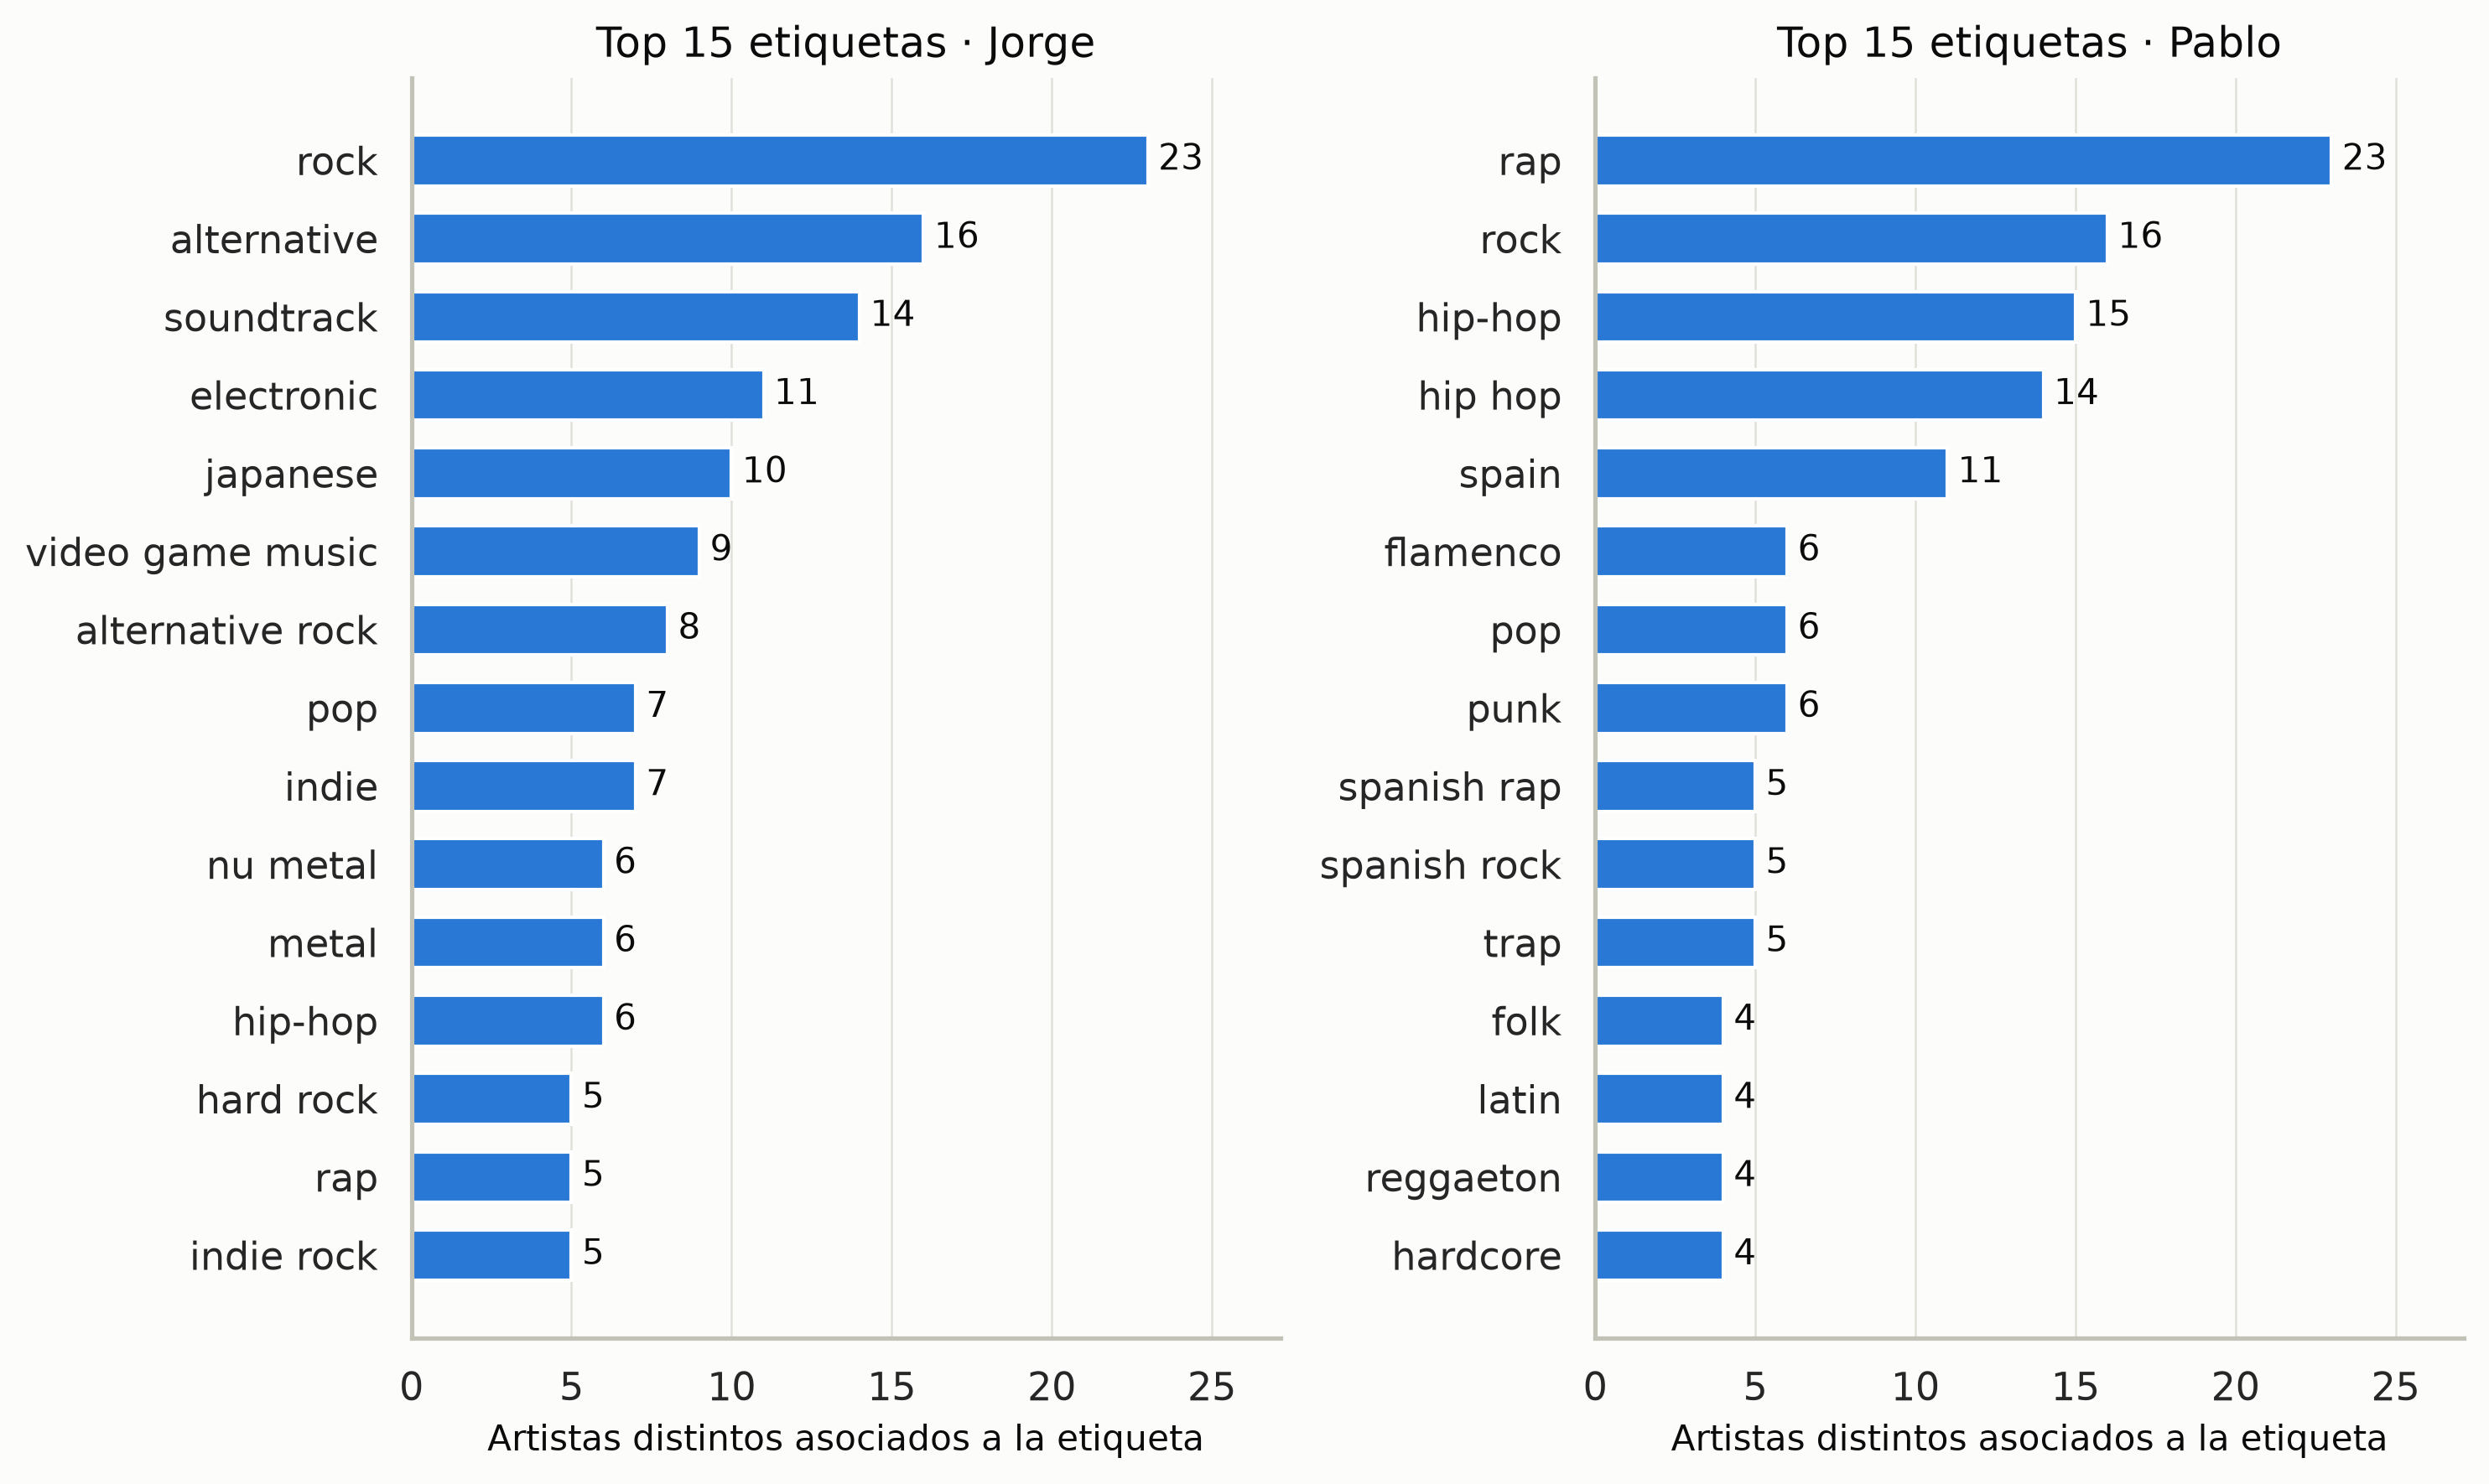
\includegraphics[width=\textwidth]{img/01_top_generos.png}
\caption{Quince etiquetas más frecuentes por usuario. Las barras horizontales facilitan leer nombres largos; ambos paneles comparten escala y muestran el número de artistas distintos.}
\label{fig:top-generos}
\end{figure}

Jorge presenta más etiquetas distintas y mayor entropía en los tres rangos: 5,3244--5,4033 bits frente a 5,0982--5,1231 en Pablo. Esto describe una distribución de etiquetas más dispersa en esta muestra, no demuestra una mayor diversidad musical objetiva: influyen el número de etiquetas por artista, sus sinónimos y la cobertura de Last.fm. La etiqueta más frecuente representa aproximadamente el 9,4--10,2\% de las asociaciones de Jorge y el 12,1--13,5\% de las de Pablo.

\begin{figure}[H]
\centering
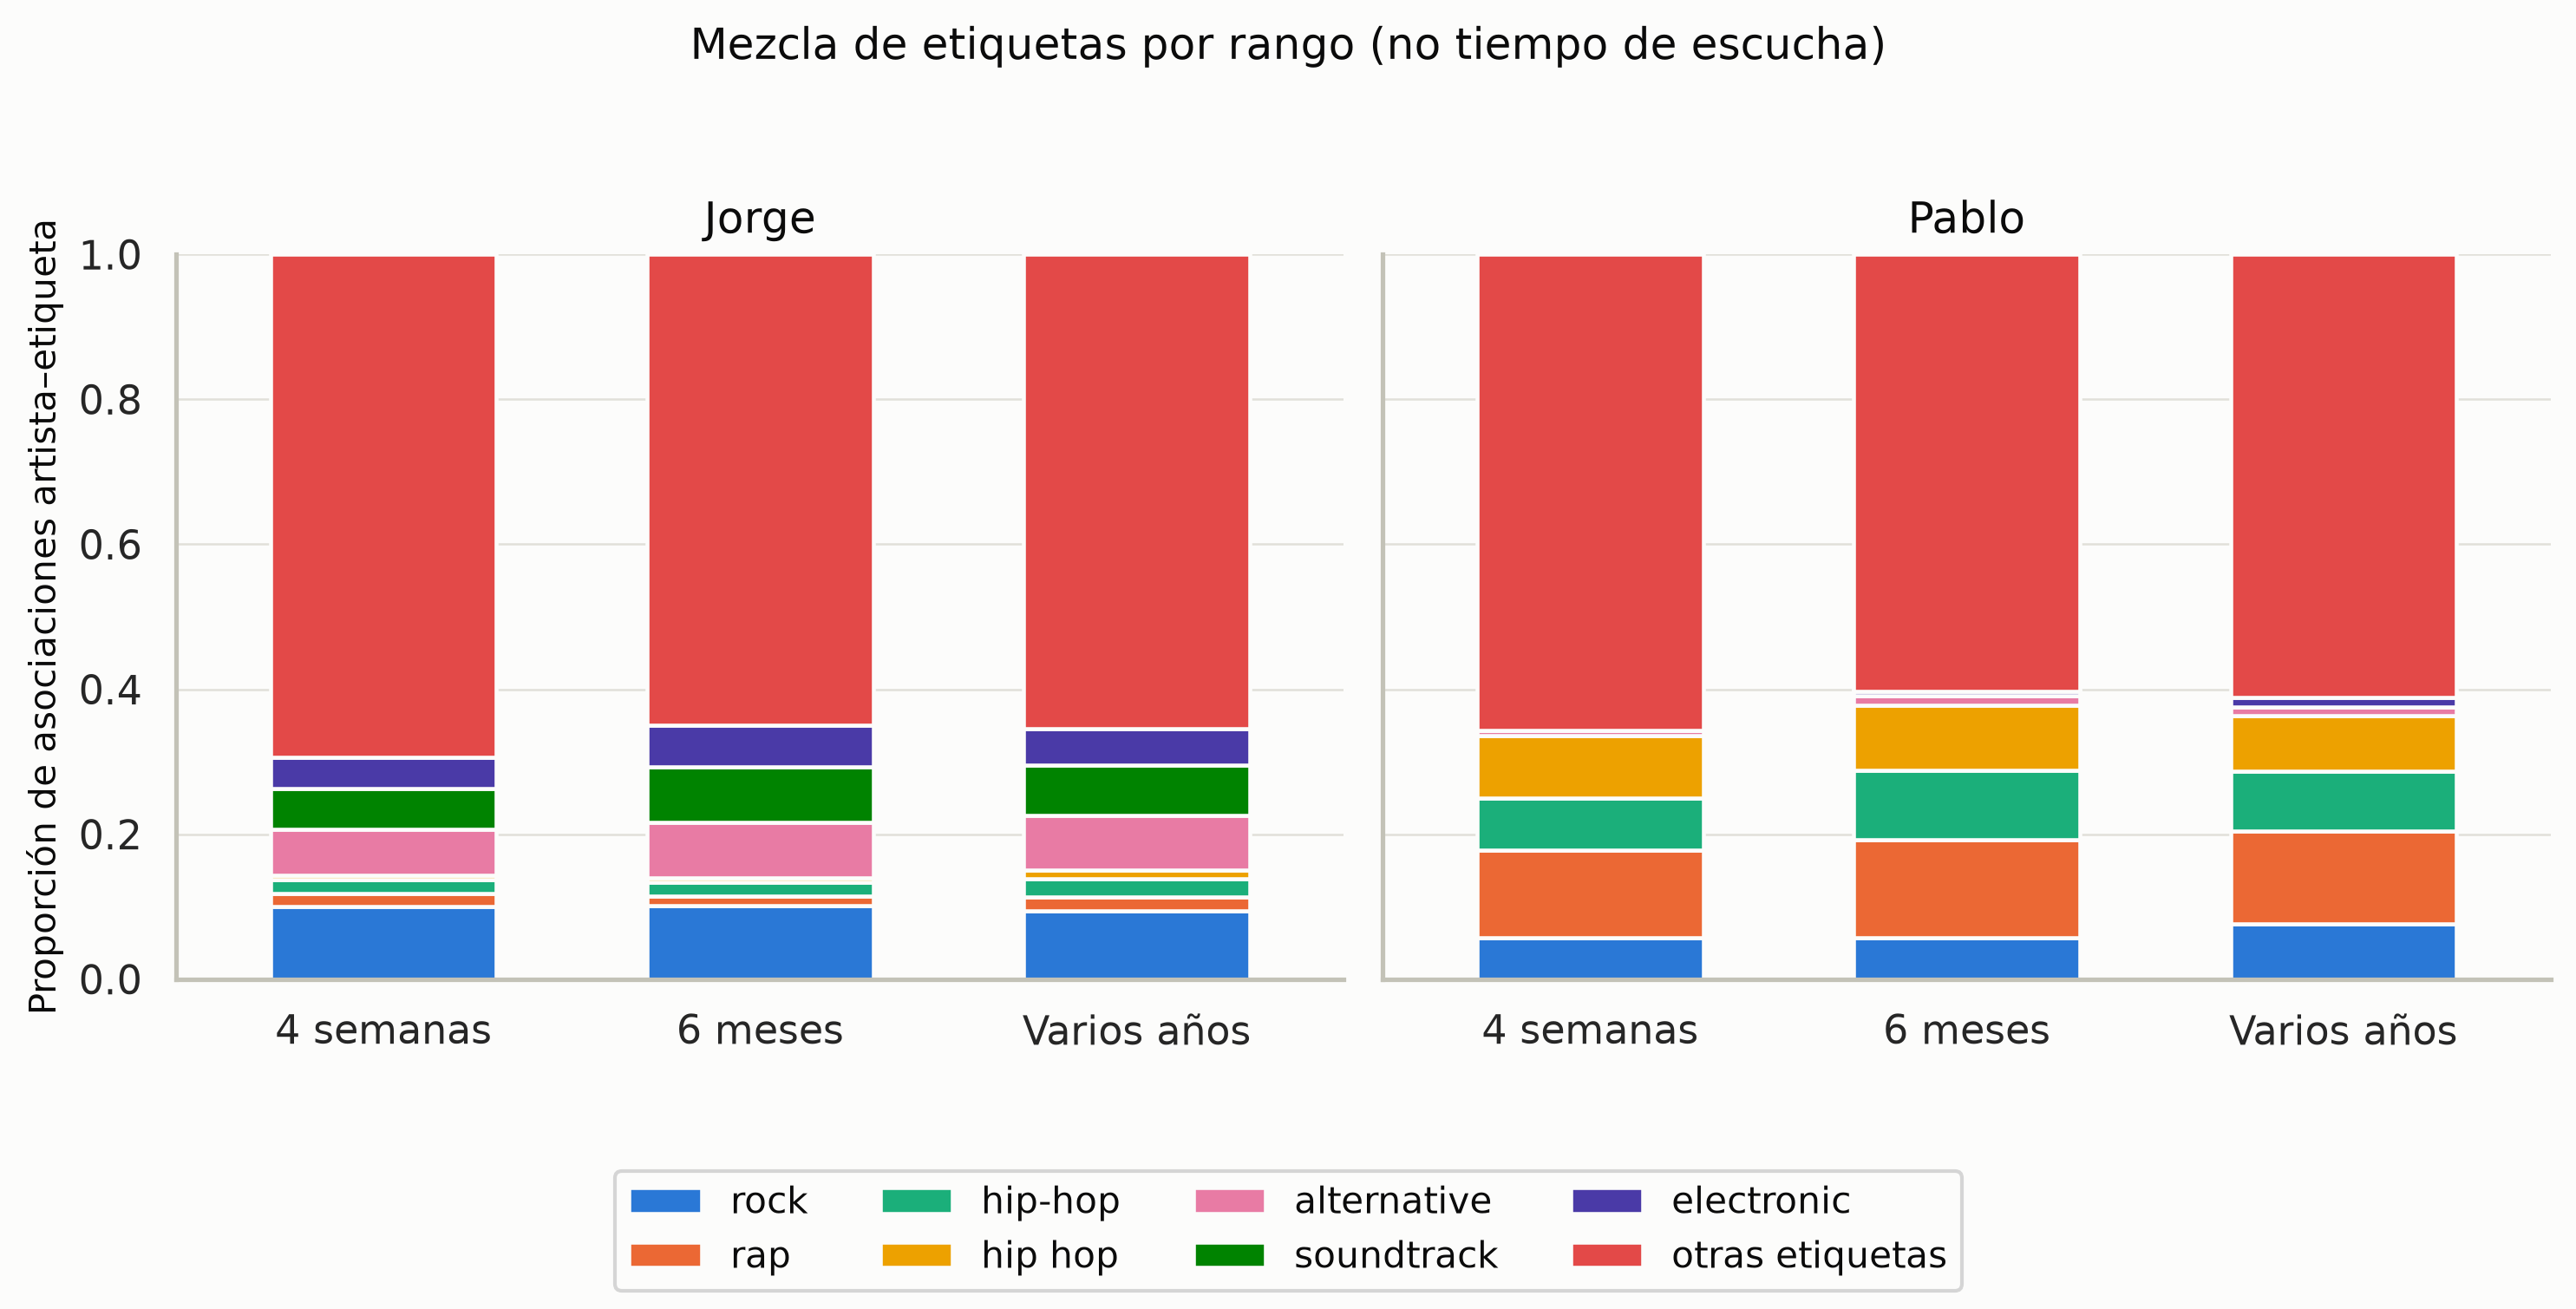
\includegraphics[width=\textwidth]{img/02_generos_por_rango.png}
\caption{Proporciones de asociaciones artista--etiqueta por rango. Las siete etiquetas destacadas y sus colores se mantienen entre paneles; el resto se agrupa. El denominador no es el tiempo de escucha.}
\label{fig:generos-rangos}
\end{figure}

\section{Coincidencia entre ventanas temporales}

Los conjuntos de artistas de cada usuario muestran coincidencias apreciables entre ventanas. Jorge tiene Jaccard de 0,5806 entre cuatro semanas y seis meses, 0,5312 entre cuatro semanas y varios años, y 0,6129 entre seis meses y varios años. Para Pablo son 0,5625, 0,5152 y 0,6667, respectivamente. En ambos casos la mayor coincidencia corresponde a medio y largo plazo.

Los cosenos de etiquetas son aún más elevados: 0,9566--0,9777 en Jorge y 0,9471--0,9717 en Pablo. La composición etiquetada es, por tanto, más parecida que la identidad exacta de los artistas. Hay 31 artistas de Jorge y 34 de Pablo presentes en los tres rangos; 25 y 32, respectivamente, aparecen en uno solo. No se interpreta esta coincidencia como una serie temporal independiente, porque las ventanas se solapan.

\begin{figure}[H]
\centering
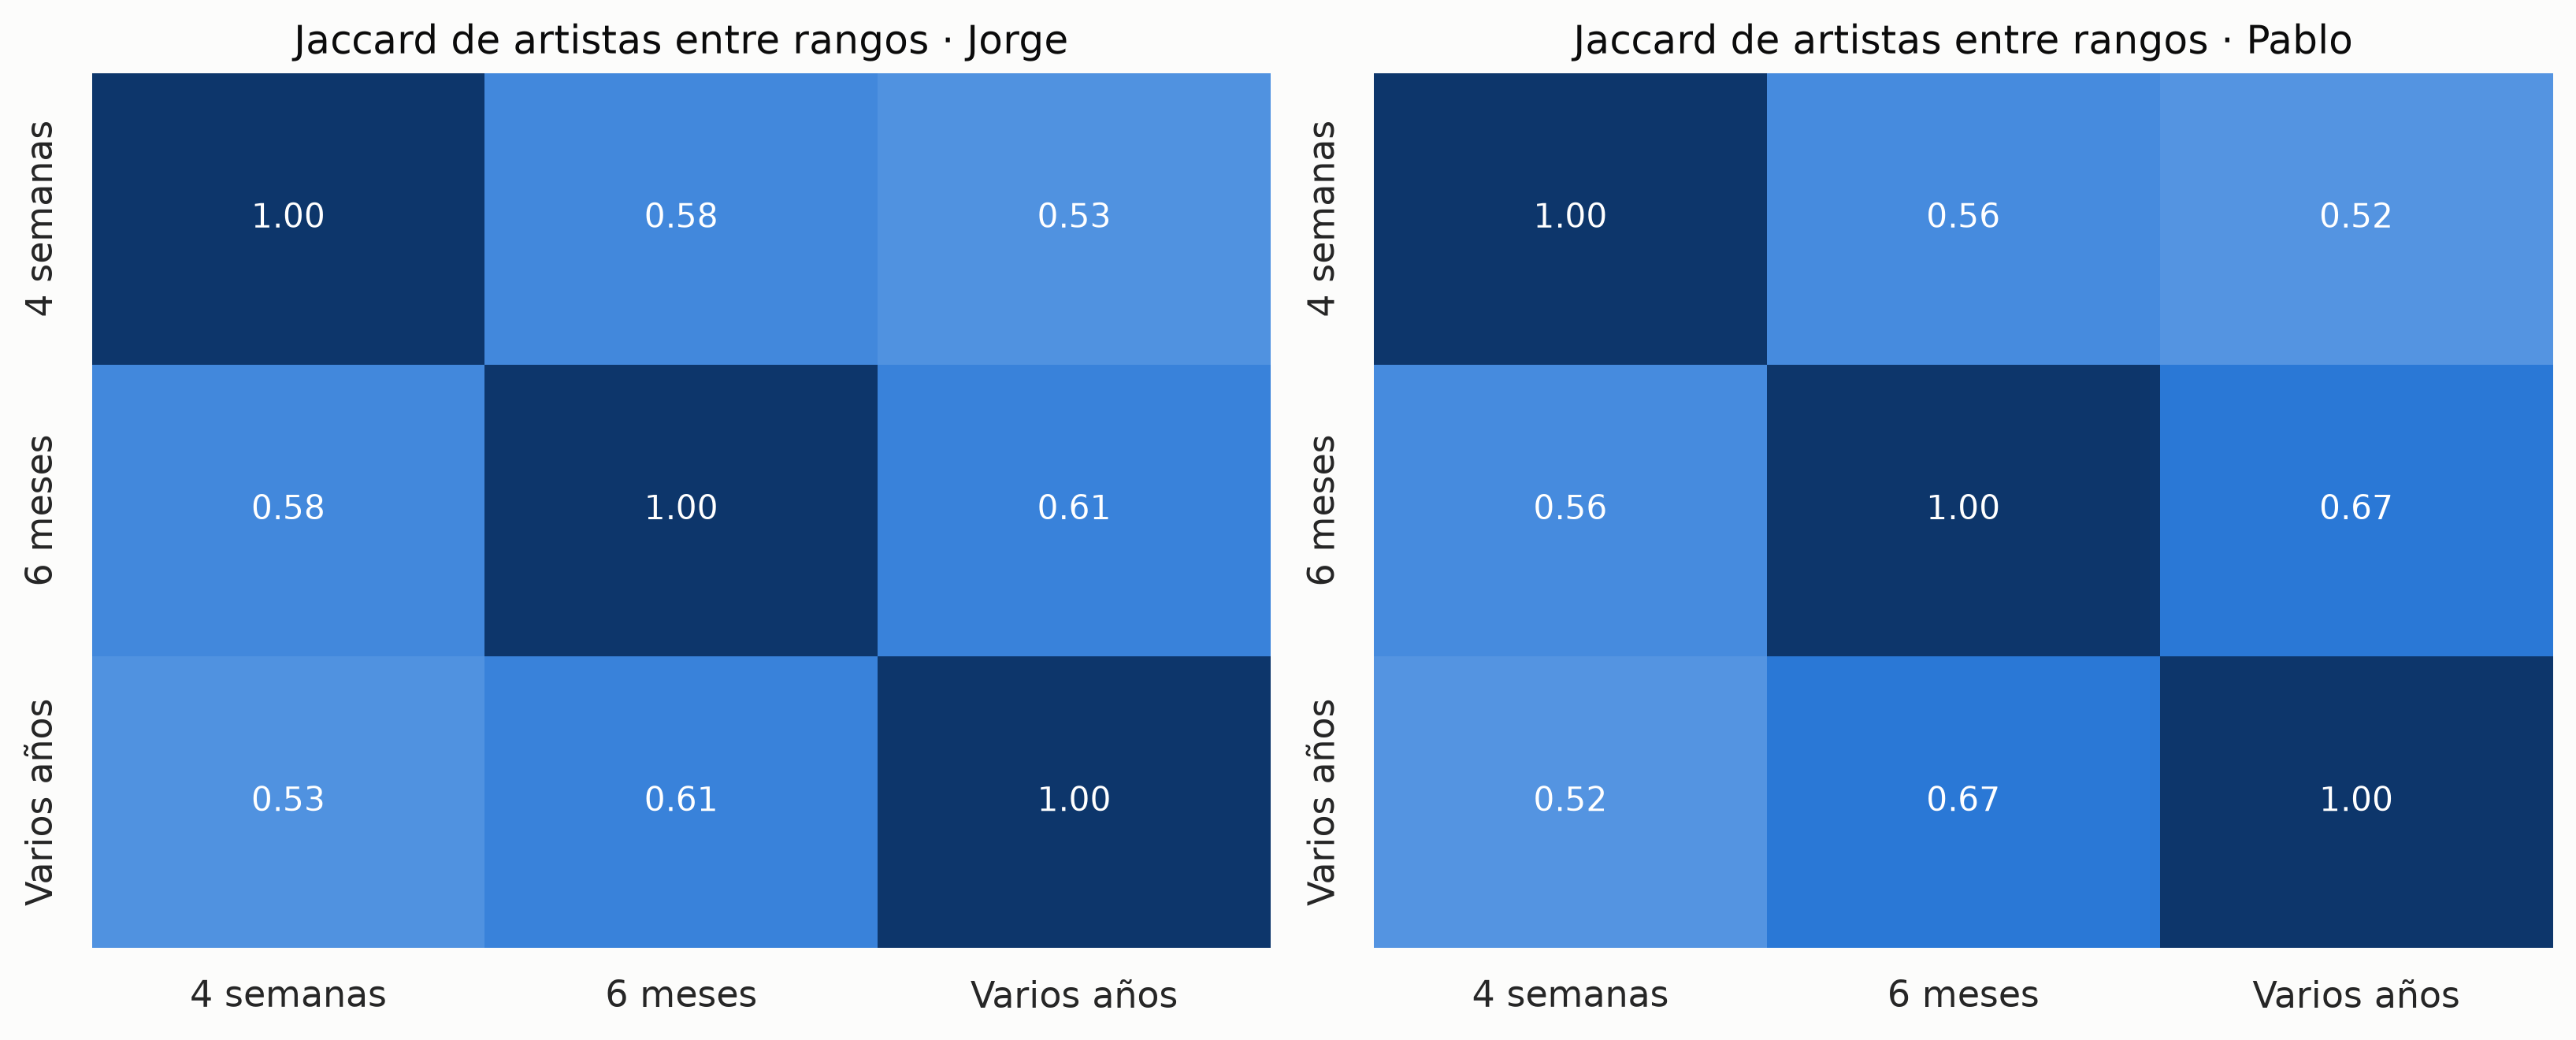
\includegraphics[width=\textwidth]{img/03_estabilidad_rangos.png}
\caption{Jaccard de artistas entre rangos, incluidos los artistas sin etiquetas. La escala común de 0 a 1 y las anotaciones permiten comparar ambas matrices; la diagonal vale 1 por construcción.}
\label{fig:estabilidad}
\end{figure}

\section{Compatibilidad entre usuarios}

La coincidencia global es de \textbf{5 artistas sobre una unión de 140}, de modo que $J=5/140=0{,}0357$. El Jaccard por ventana permanece entre 0,0309 y 0,0417. La similitud del coseno de etiquetas es mayor: 0,3247 en cuatro semanas, 0,3110 en seis meses y 0,4112 en varios años; al reunir las tres ventanas alcanza 0,4686, con 27 etiquetas comunes. No son porcentajes equivalentes de compatibilidad: Jaccard compara identidades y el coseno compara composiciones etiquetadas.

\begin{table}[H]
\centering
\begin{tabular}{lrrr}
\hline
Rango & Artistas comunes & Jaccard & Coseno \\
\hline
4 semanas & 3 & 0,0316 & 0,3247 \\
6 meses & 4 & 0,0417 & 0,3110 \\
Varios años & 3 & 0,0309 & 0,4112 \\
Global & 5 & 0,0357 & 0,4686 \\
\hline
\end{tabular}
\caption{Dos medidas complementarias de coincidencia entre usuarios. Los artistas sin etiquetas se mantienen en el cálculo de Jaccard.}
\label{tab:compatibilidad}
\end{table}

\begin{figure}[H]
\centering
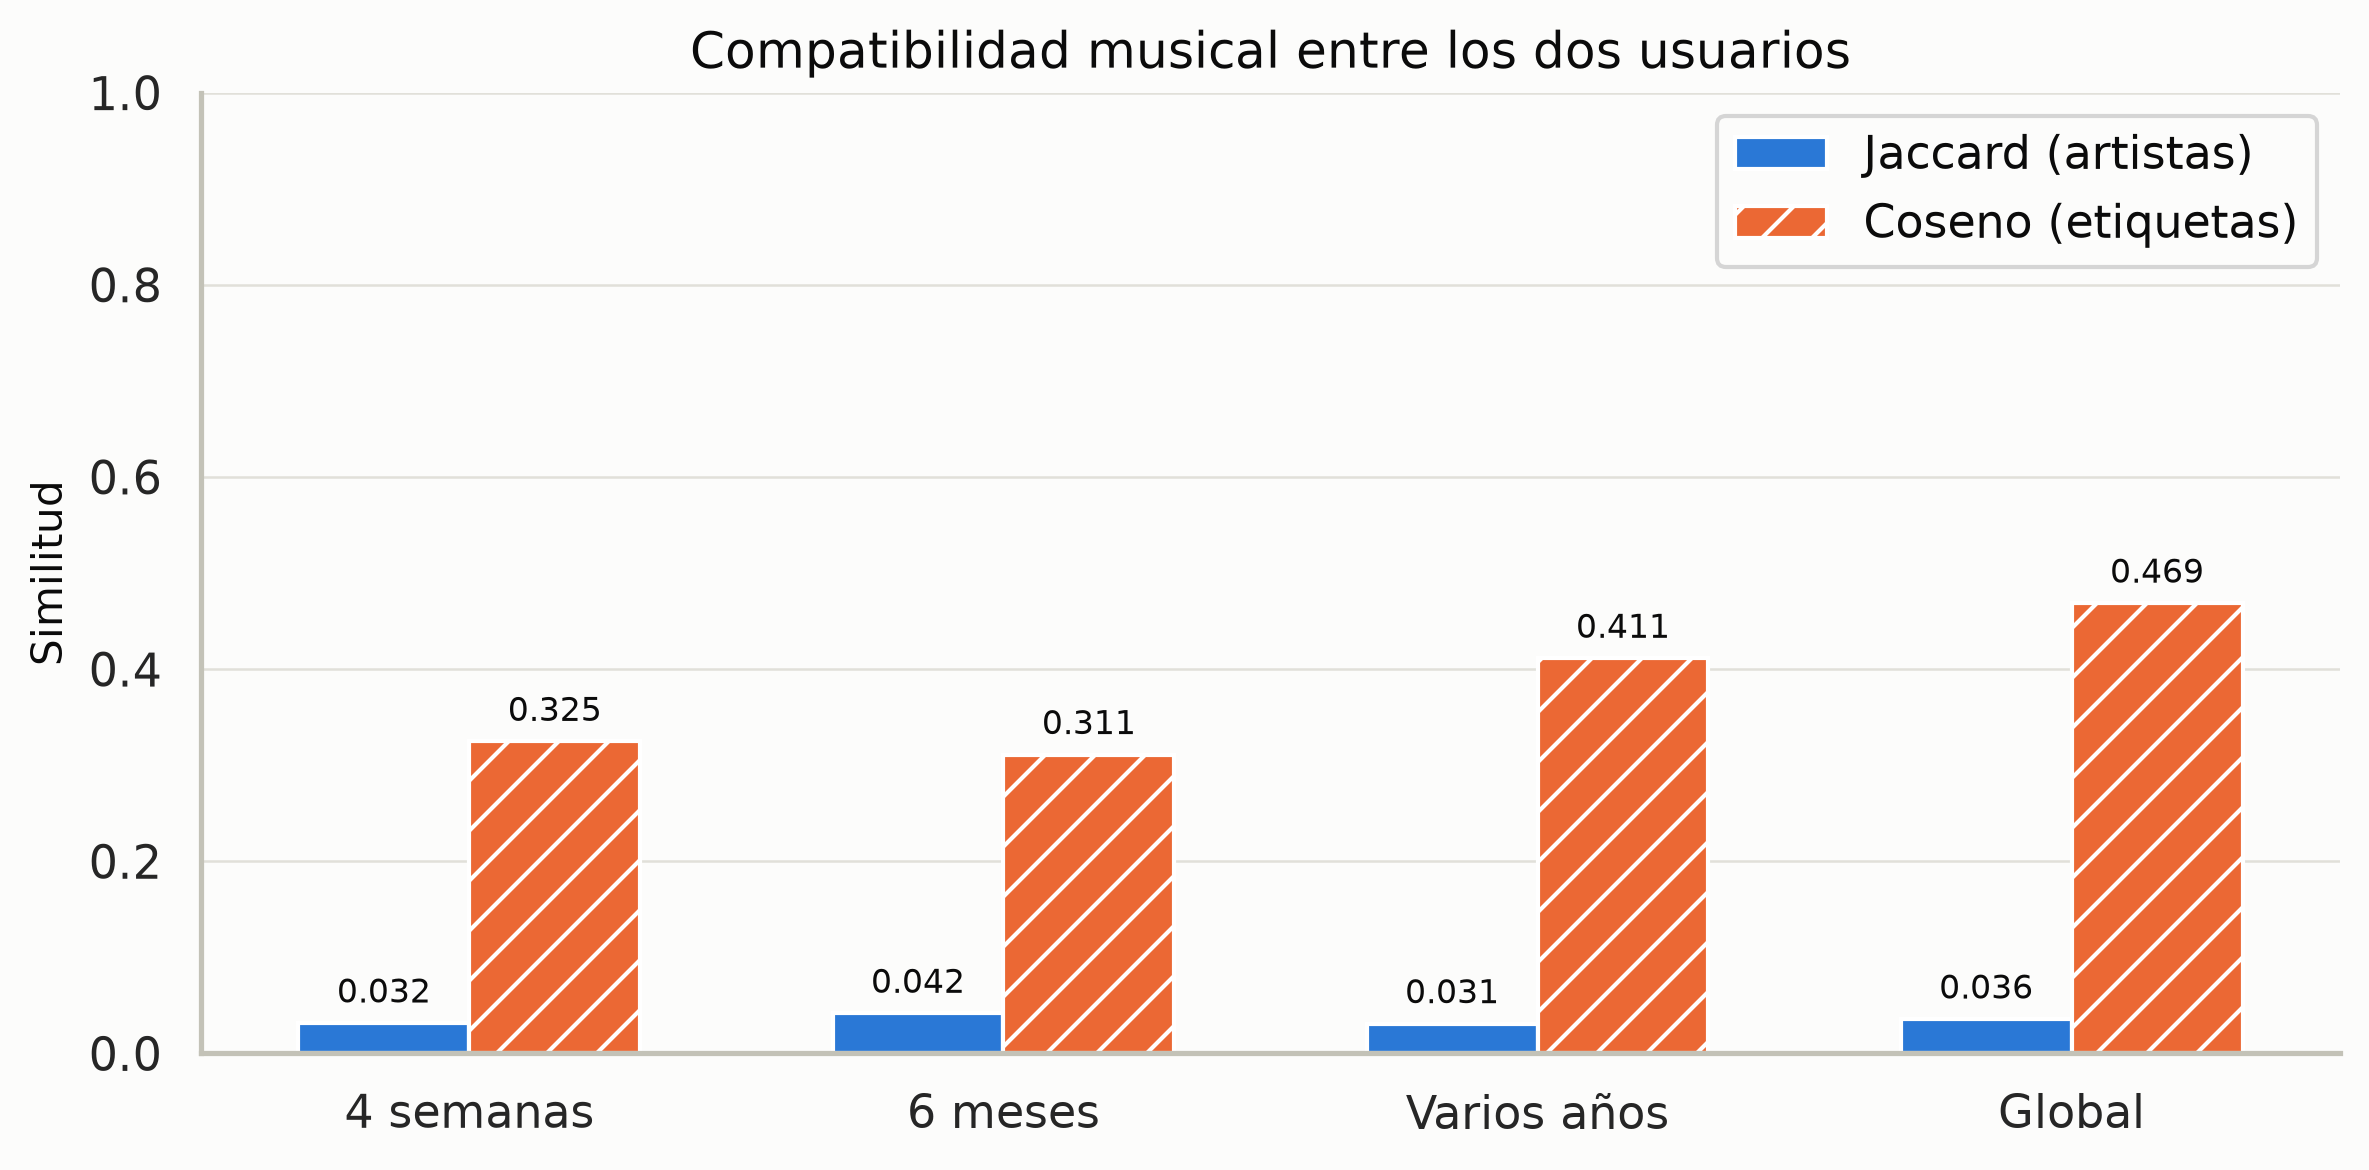
\includegraphics[width=\textwidth]{img/04_compatibilidad.png}
\caption{Jaccard de artistas y coseno de etiquetas por ventana y global. Se conserva una escala común 0--1 y se distinguen las métricas mediante leyenda y trama, además del color.}
\label{fig:compatibilidad}
\end{figure}

El resultado permite afirmar que las listas concretas son muy distintas, pero comparten parte del vocabulario musical, incluido \texttt{rock}. La diferencia entre medidas es coherente con que dos personas escuchen artistas distintos vinculados a etiquetas semejantes. No se transforma el coseno en una valoración personal ni en una probabilidad de compartir gustos.

\section{Cobertura de las fuentes y tratamiento de ausencias}

El enriquecimiento se completó el 4 de noviembre de 2026. Last.fm devuelve oyentes, reproducciones y al menos un vecino para los 140 artistas del historial. Esto no implica cobertura perfecta de todos sus atributos: faltan 20 identificadores MusicBrainz. Deezer aporta fans y número de álbumes para 136 artistas con coincidencia exacta de nombre; los cuatro restantes se mantienen ausentes, sin atribuirles resultados aproximados.

\begin{table}[H]
\centering
\begin{tabular}{lrr}
\hline
Información ausente & Artistas & Porcentaje \\
\hline
Etiquetas del CSV & 5 & 3,57\% \\
Oyentes Last.fm & 0 & 0,00\% \\
Reproducciones Last.fm & 0 & 0,00\% \\
Identificador MusicBrainz & 20 & 14,29\% \\
Sin vecinos similares & 0 & 0,00\% \\
Fans Deezer & 4 & 2,86\% \\
Álbumes Deezer & 4 & 2,86\% \\
\hline
\end{tabular}
\caption{Ausencias sobre los 140 artistas únicos. Los campos no son excluyentes: un artista puede carecer de varios atributos.}
\label{tab:cobertura-resultados}
\end{table}

\begin{figure}[H]
\centering
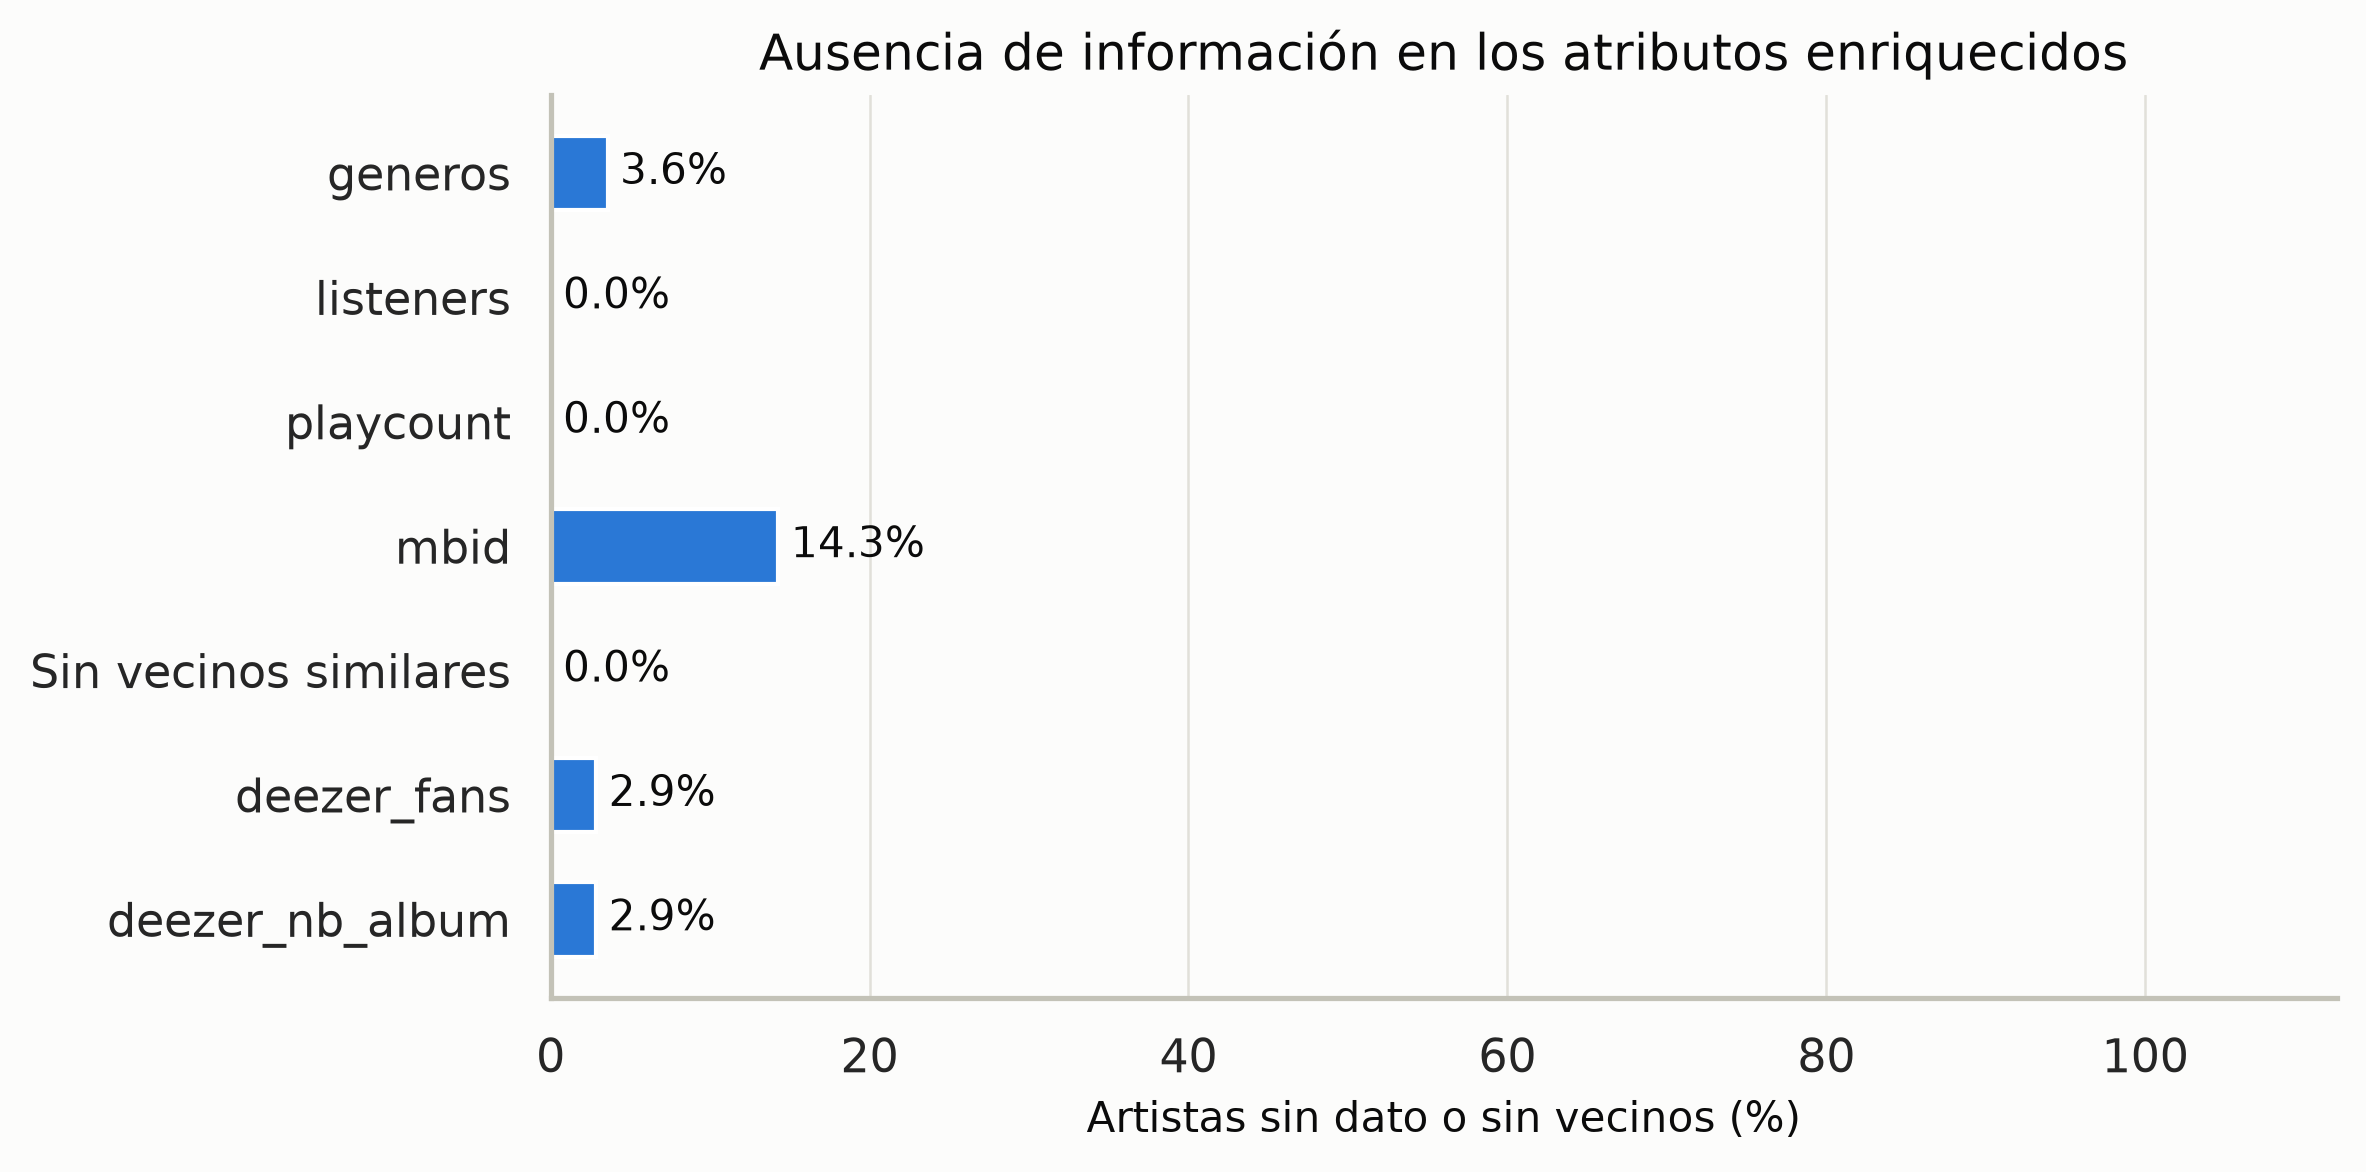
\includegraphics[width=\textwidth]{img/09_nulos.png}
\caption{Porcentaje sin información por atributo. Las barras parten de cero y tienen una escala porcentual común; ``sin vecinos'' cuenta listas vacías, no solo nulos de almacenamiento.}
\label{fig:nulos}
\end{figure}

El procedimiento de imputación no modifica ningún valor de oyentes o reproducciones, porque están completos. Genera cuatro valores de fans en una columna separada, según las reglas de mediana descritas en el Capítulo~\ref{chap:modelo}; la mediana global observada de fans es 16\,042,5. Las columnas originales y las banderas de imputación se conservan. Los análisis siguientes usan observaciones reales: la correlación entre fuentes tiene 136 casos, no 140.

\section{Popularidad externa y posición personal}

\begin{table}[H]
\centering
\begin{tabular}{llrrr}
\hline
Usuario & Rango & $n$ & Spearman $\rho$ & Valor $p$ \\
\hline
Jorge & 4 semanas & 48 & 0,1845 & 0,2092 \\
Jorge & 6 meses & 50 & $-0{,}0033$ & 0,9818 \\
Jorge & Varios años & 50 & $-0{,}0337$ & 0,8165 \\
Pablo & 4 semanas & 50 & $-0{,}1055$ & 0,4659 \\
Pablo & 6 meses & 50 & 0,2548 & 0,0741 \\
Pablo & Varios años & 50 & 0,3275 & 0,0202 \\
\hline
\end{tabular}
\caption{Correlación entre posición numérica y logaritmo de oyentes de Last.fm, solo con casos observados. Los valores $p$ son exploratorios y no están corregidos por las seis comparaciones.}
\label{tab:popularidad}
\end{table}

No aparece una asociación de igual signo y magnitud en los seis perfiles. La mayor correlación es la de Pablo en varios años ($\rho=0{,}3275$): al aumentar la posición numérica, es decir, al bajar en el ranking, tiende a aumentar la popularidad externa. No significa que los artistas más populares estén mejor situados, sino lo contrario. Su valor $p$ sin ajustar es 0,0202, pero se han examinado seis combinaciones y no existe un diseño confirmatorio; tampoco las ventanas son independientes. El resultado se describe como una asociación moderada y localizada, sin generalizar una preferencia estable o causal.

\begin{figure}[H]
\centering
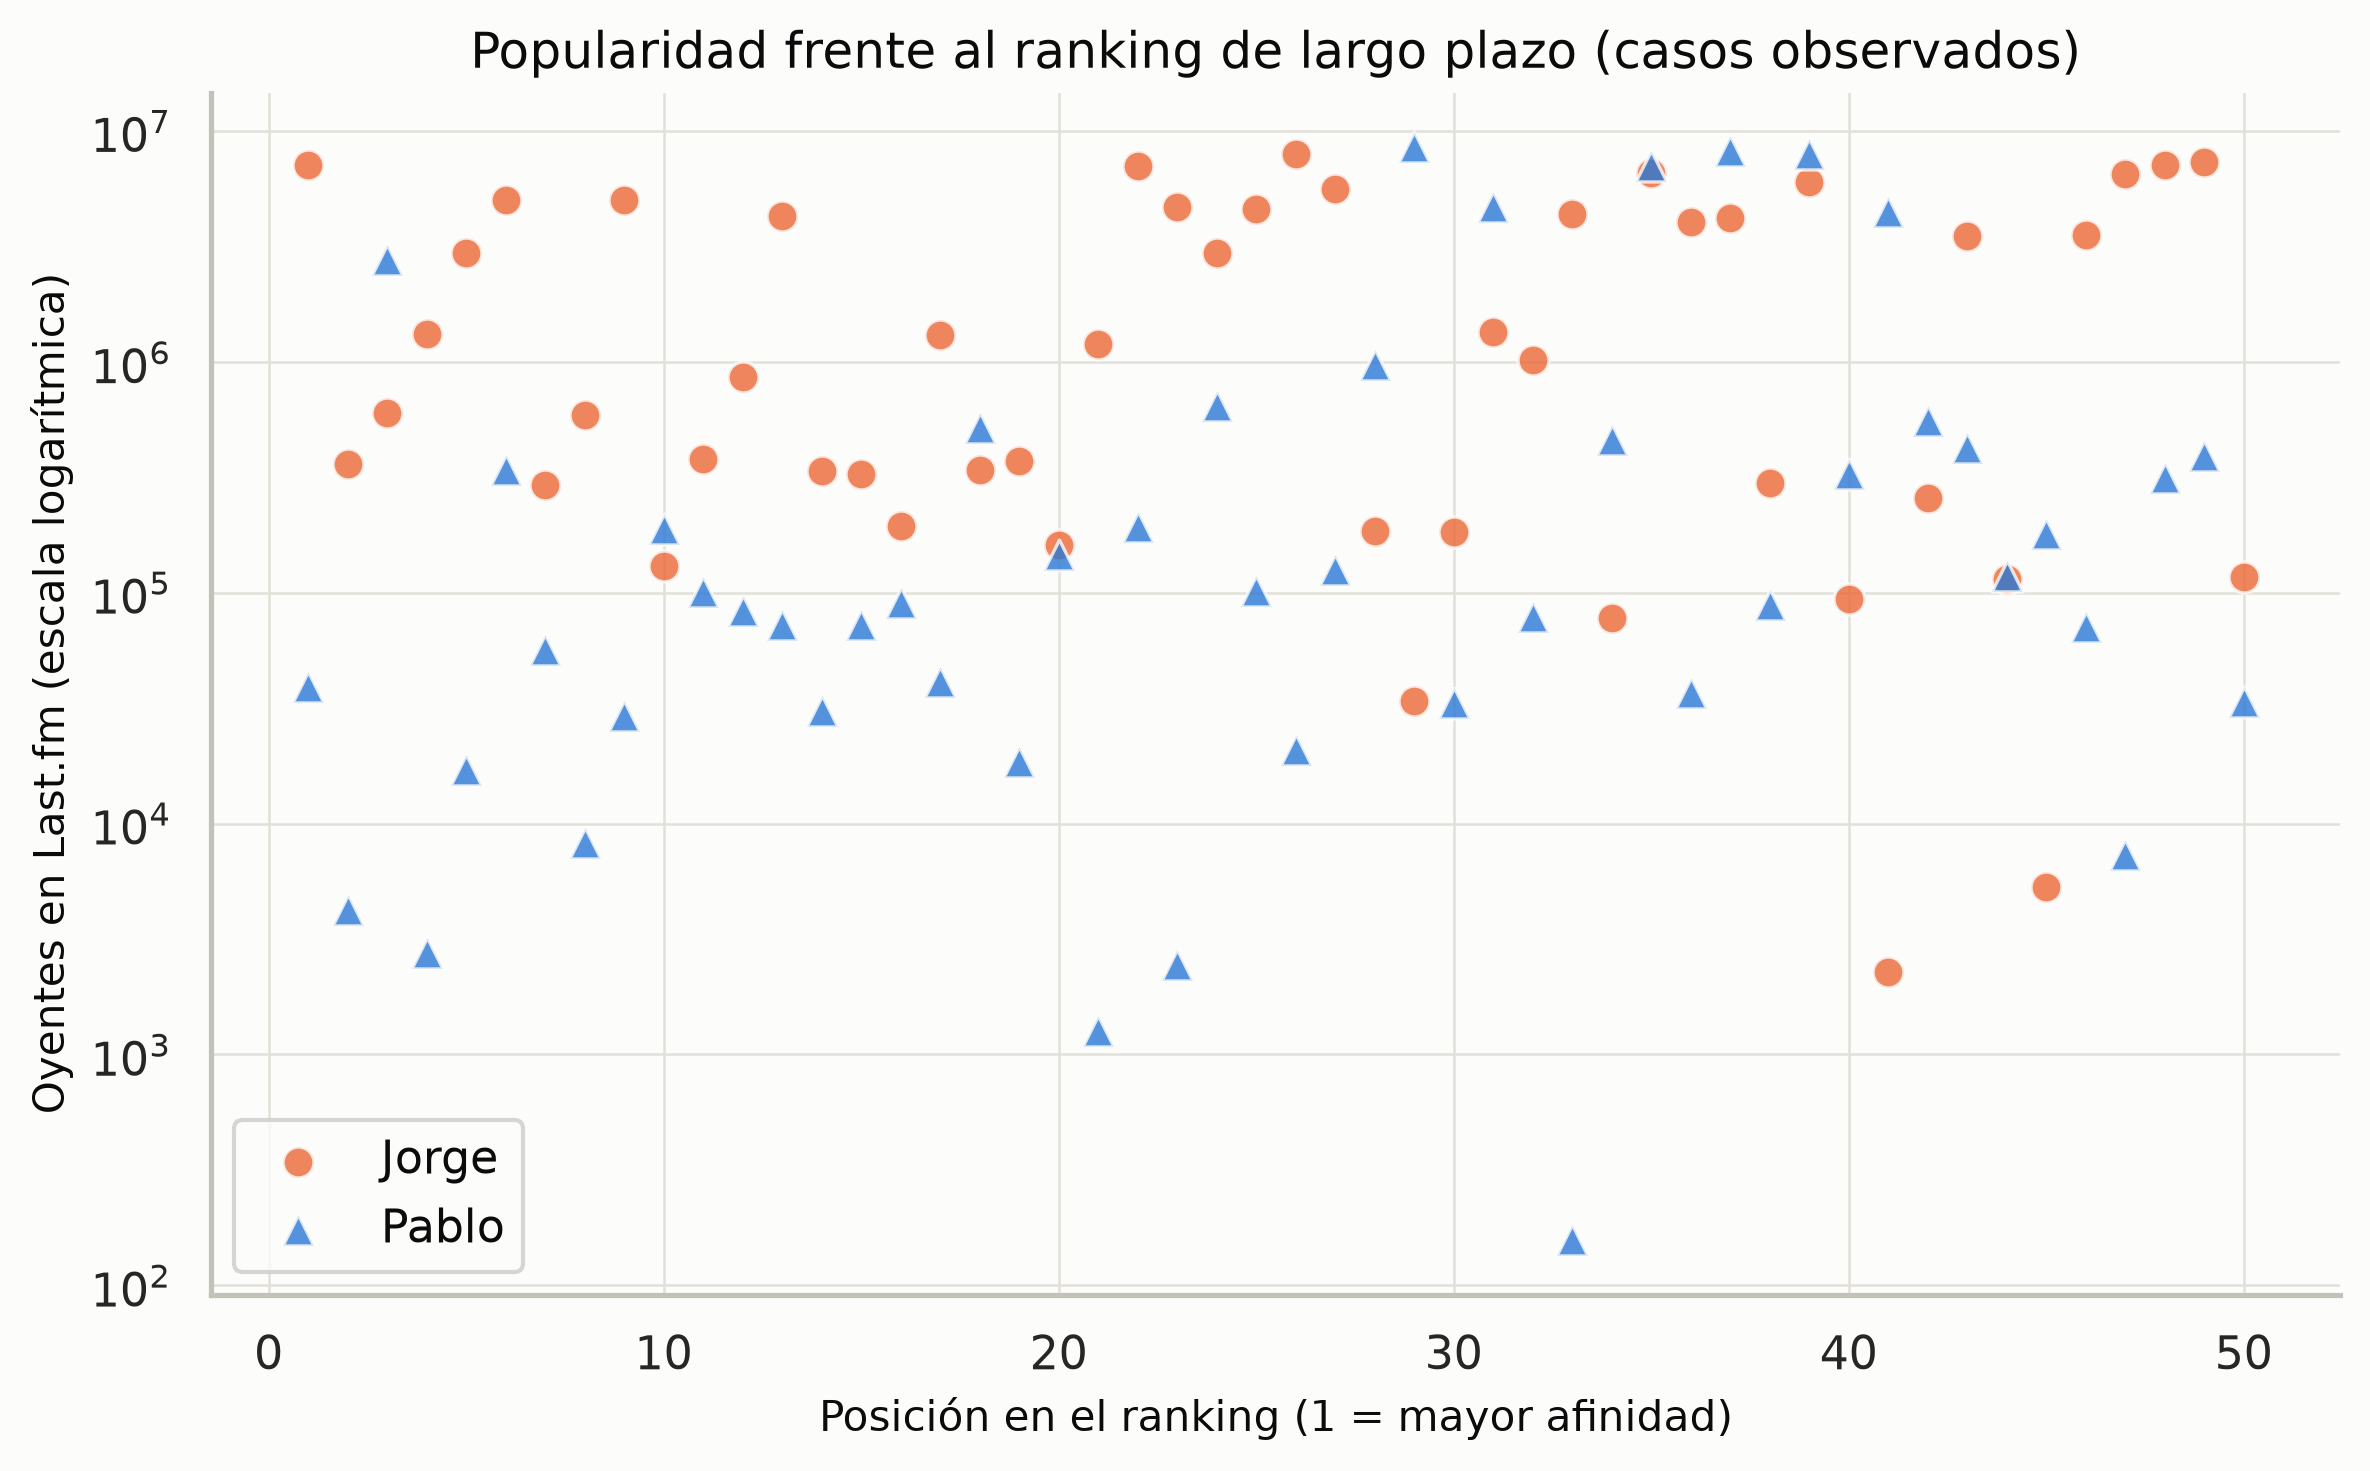
\includegraphics[width=\textwidth]{img/05_popularidad_rank.png}
\caption{Oyentes externos frente a posición personal en la ventana larga. La escala logarítmica permite representar varios órdenes de magnitud; usuario y forma de los puntos se mantienen identificados en la leyenda. Cada punto es una entrada del ranking, no una reproducción.}
\label{fig:popularidad}
\end{figure}

Entre las dos medidas externas de popularidad, oyentes de Last.fm y fans de Deezer, se obtiene $\rho=0{,}6830$ con 136 pares observados ($p\simeq5{,}19\times10^{-20}$). La relación positiva indica ordenaciones parcialmente concordantes dentro del conjunto seleccionado, pero no intercambiabilidad: son plataformas y acciones de usuario distintas. No se utiliza esta asociación para rellenar los cuatro fans ausentes ni se presenta como representativa de todos los artistas de ambas plataformas.

\section{Afinidad de candidatos nuevos}

Se generan 20 candidatos fuera de los dos historiales y se consultan sus propios vecinos. Los \textbf{20 son puntuables para ambos usuarios}; esta cobertura se refiere a la disponibilidad del cálculo, no a que encajen con ambos perfiles. De hecho, \textbf{ninguno de los veinte obtiene puntuación positiva para los dos usuarios a la vez}. Cada uno presenta solapamiento ponderado con un perfil y cero con el otro.

La Figura~\ref{fig:afinidad} muestra diez candidatos ordenados por la media de sus dos puntuaciones, con identificadores anónimos. El candidato C01 obtiene 0,2175 en Jorge y 0 en Pablo; C02 obtiene 0 y 0,2156, respectivamente. Sus medias, 0,1087 y 0,1078, no representan una afinidad compartida. La media prioriza una puntuación unilateral relativamente alta, de modo que no debe interpretarse este top como una selección de consenso. Un cero significa ausencia de vecinos coincidentes en el historial truncado, no rechazo declarado del artista.

\begin{figure}[H]
\centering
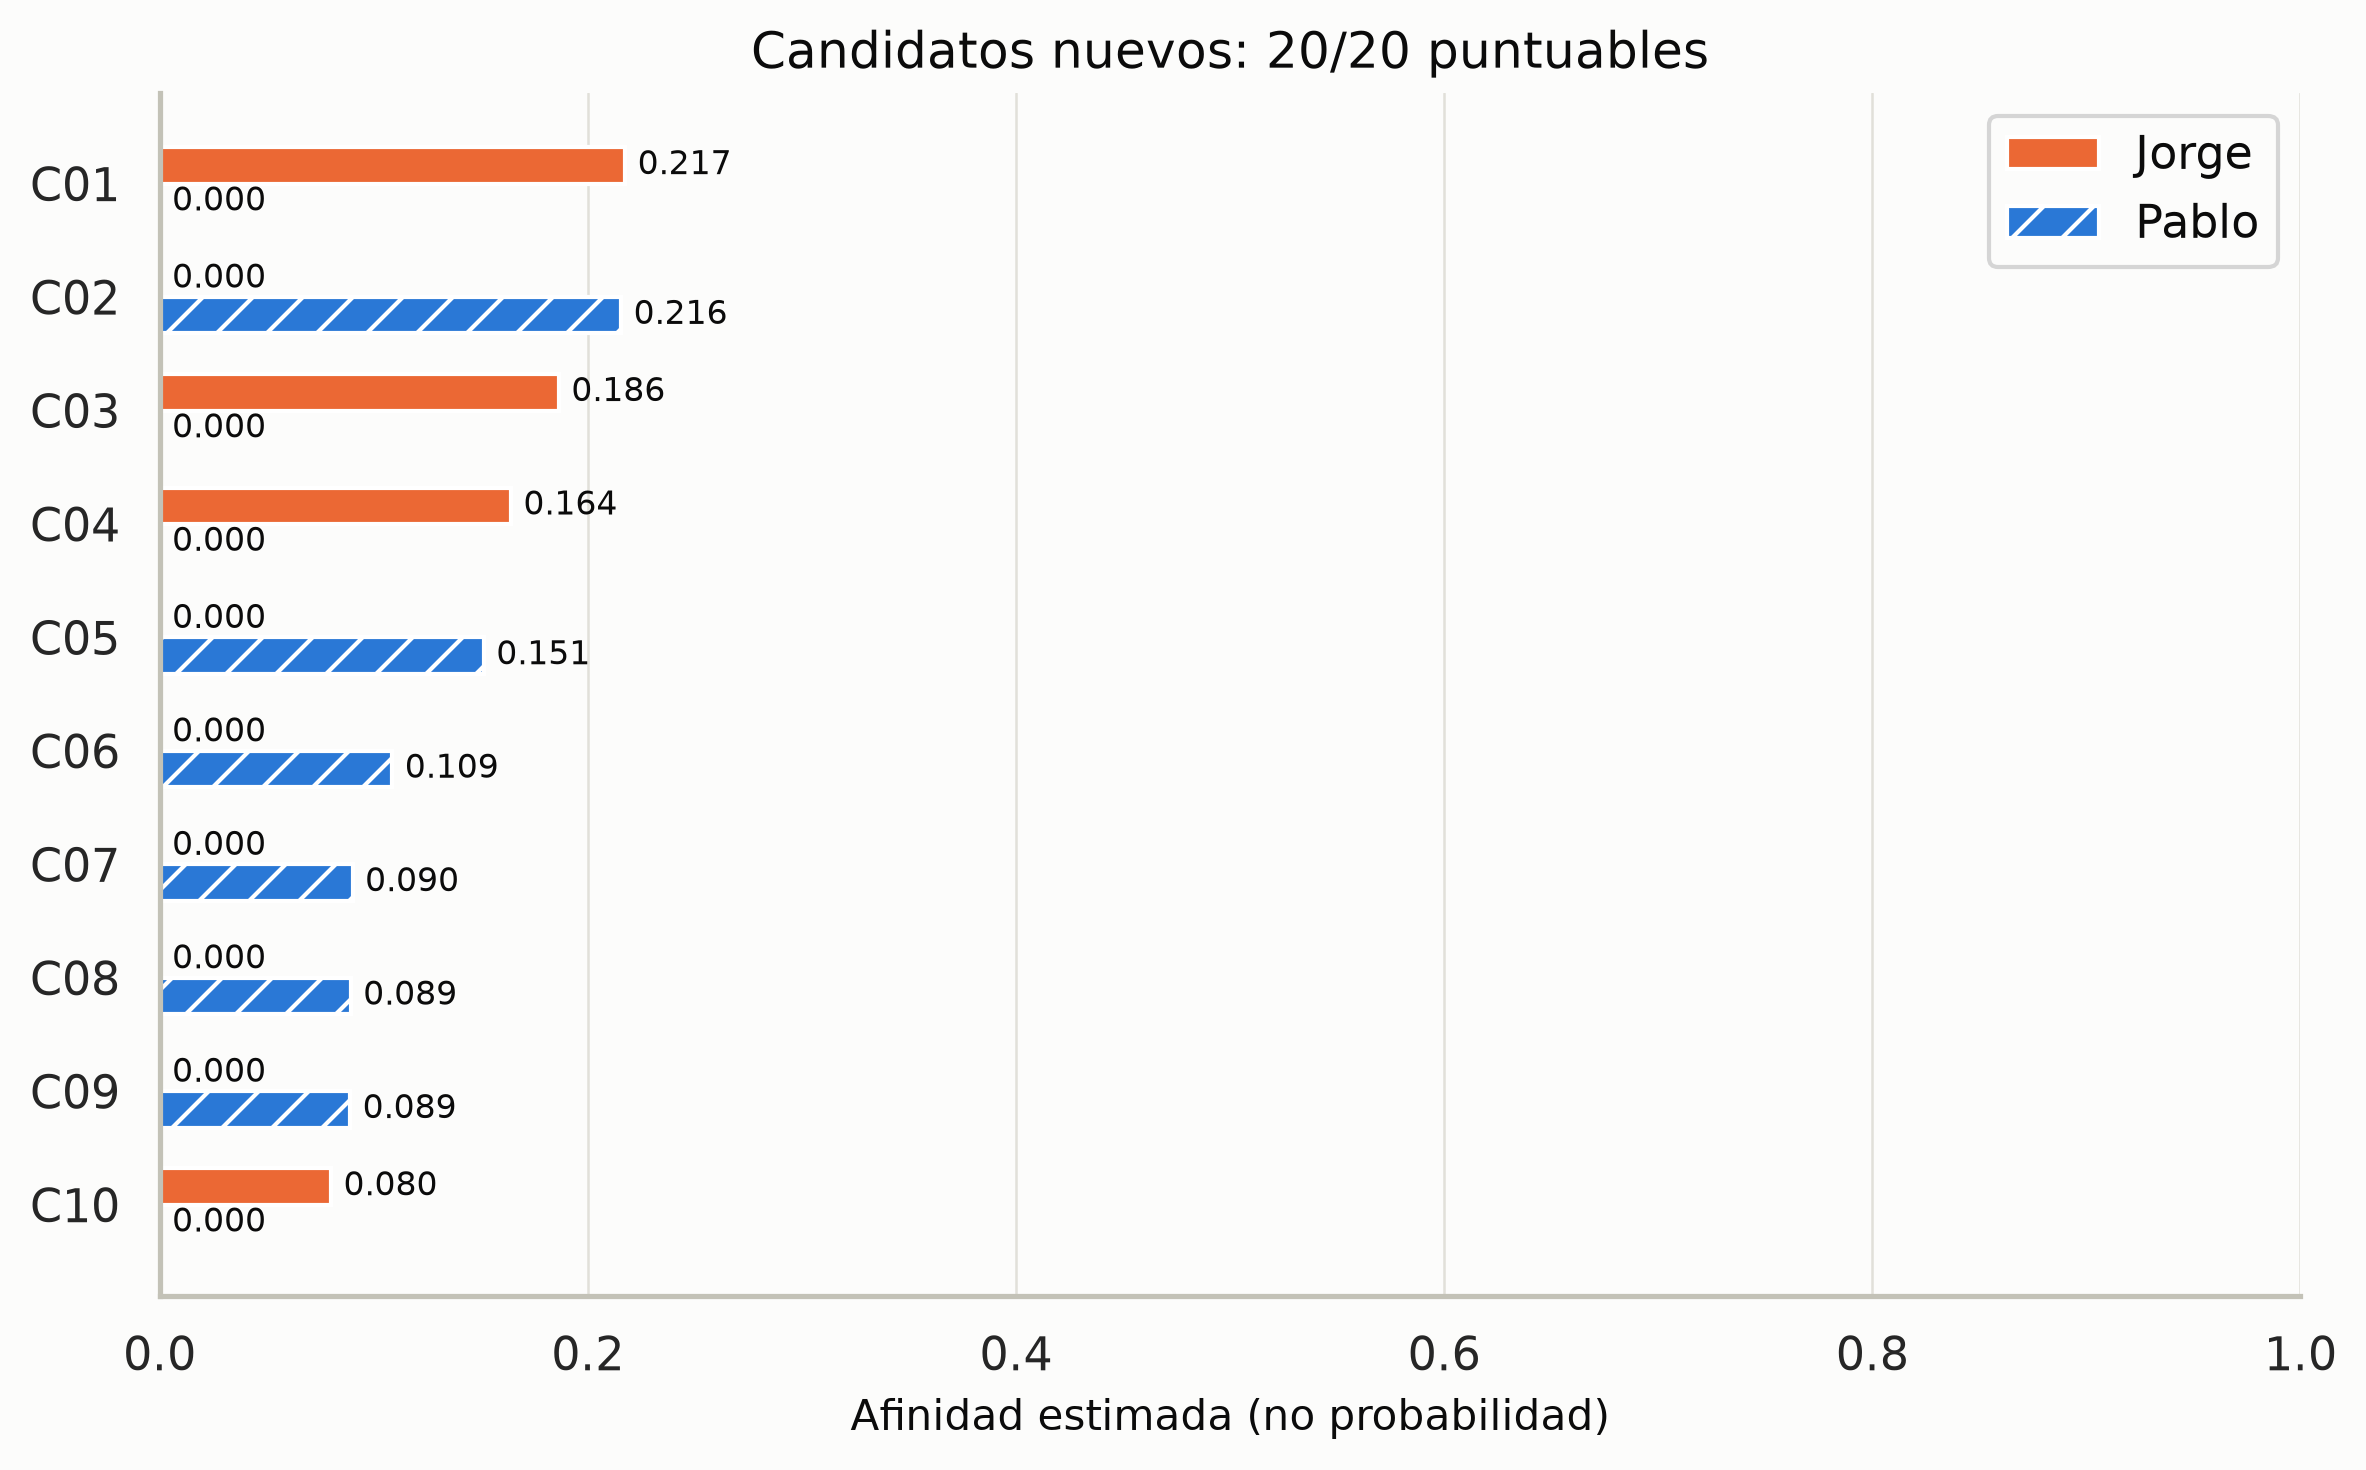
\includegraphics[width=\textwidth]{img/06_afinidad.png}
\caption{Diez candidatos anónimos con mayor afinidad media. El eje común 0--1, las etiquetas numéricas y la trama permiten ver tanto las diferencias como los ceros. La cobertura 20/20 indica que el cálculo está disponible, no una tasa de acierto.}
\label{fig:afinidad}
\end{figure}

\begin{table}[H]
\centering
\small
\begin{tabular}{lrrrrr}
\hline
Usuario & Ocultos & Controles & Mediana ocultos & Mediana controles & Valor $p$ \\
\hline
Jorge & 10 & 20 & 0,1069 & 0,0435 & 0,0801 \\
Pablo & 10 & 20 & 0,1647 & 0,0000 & 0,000205 \\
\hline
\end{tabular}
\caption{Comprobación exploratoria \emph{leave-one-out}. El valor $p$ corresponde a la prueba U unilateral (ocultos mayores que controles); los controles no son ejemplos negativos ni una muestra independiente.}
\label{tab:loo}
\end{table}

Las medianas de los favoritos ocultos son mayores que las de los candidatos-control en ambos usuarios. Los estadísticos U son 132,0 en Jorge y 177,5 en Pablo. Esta comparación muestra el comportamiento interno de la heurística, pero no proporciona precisión, tasa de acierto ni garantía de que gusten las recomendaciones: candidatos y favoritos comparten el mecanismo de selección y no se dispone de valoraciones independientes.

\section{Agrupamiento exploratorio}
\label{sec:resultados-clustering}

De los 140 artistas, cinco carecen de etiquetas y otros dos quedan sin ninguna tras exigir soporte mínimo de dos artistas por etiqueta. La matriz final tiene \textbf{133 artistas y 52 etiquetas}; se descartan 78 etiquetas de soporte uno. Esta selección limita la representación de estilos raros y debe tenerse en cuenta al interpretar los grupos.

\begin{figure}[H]
\centering
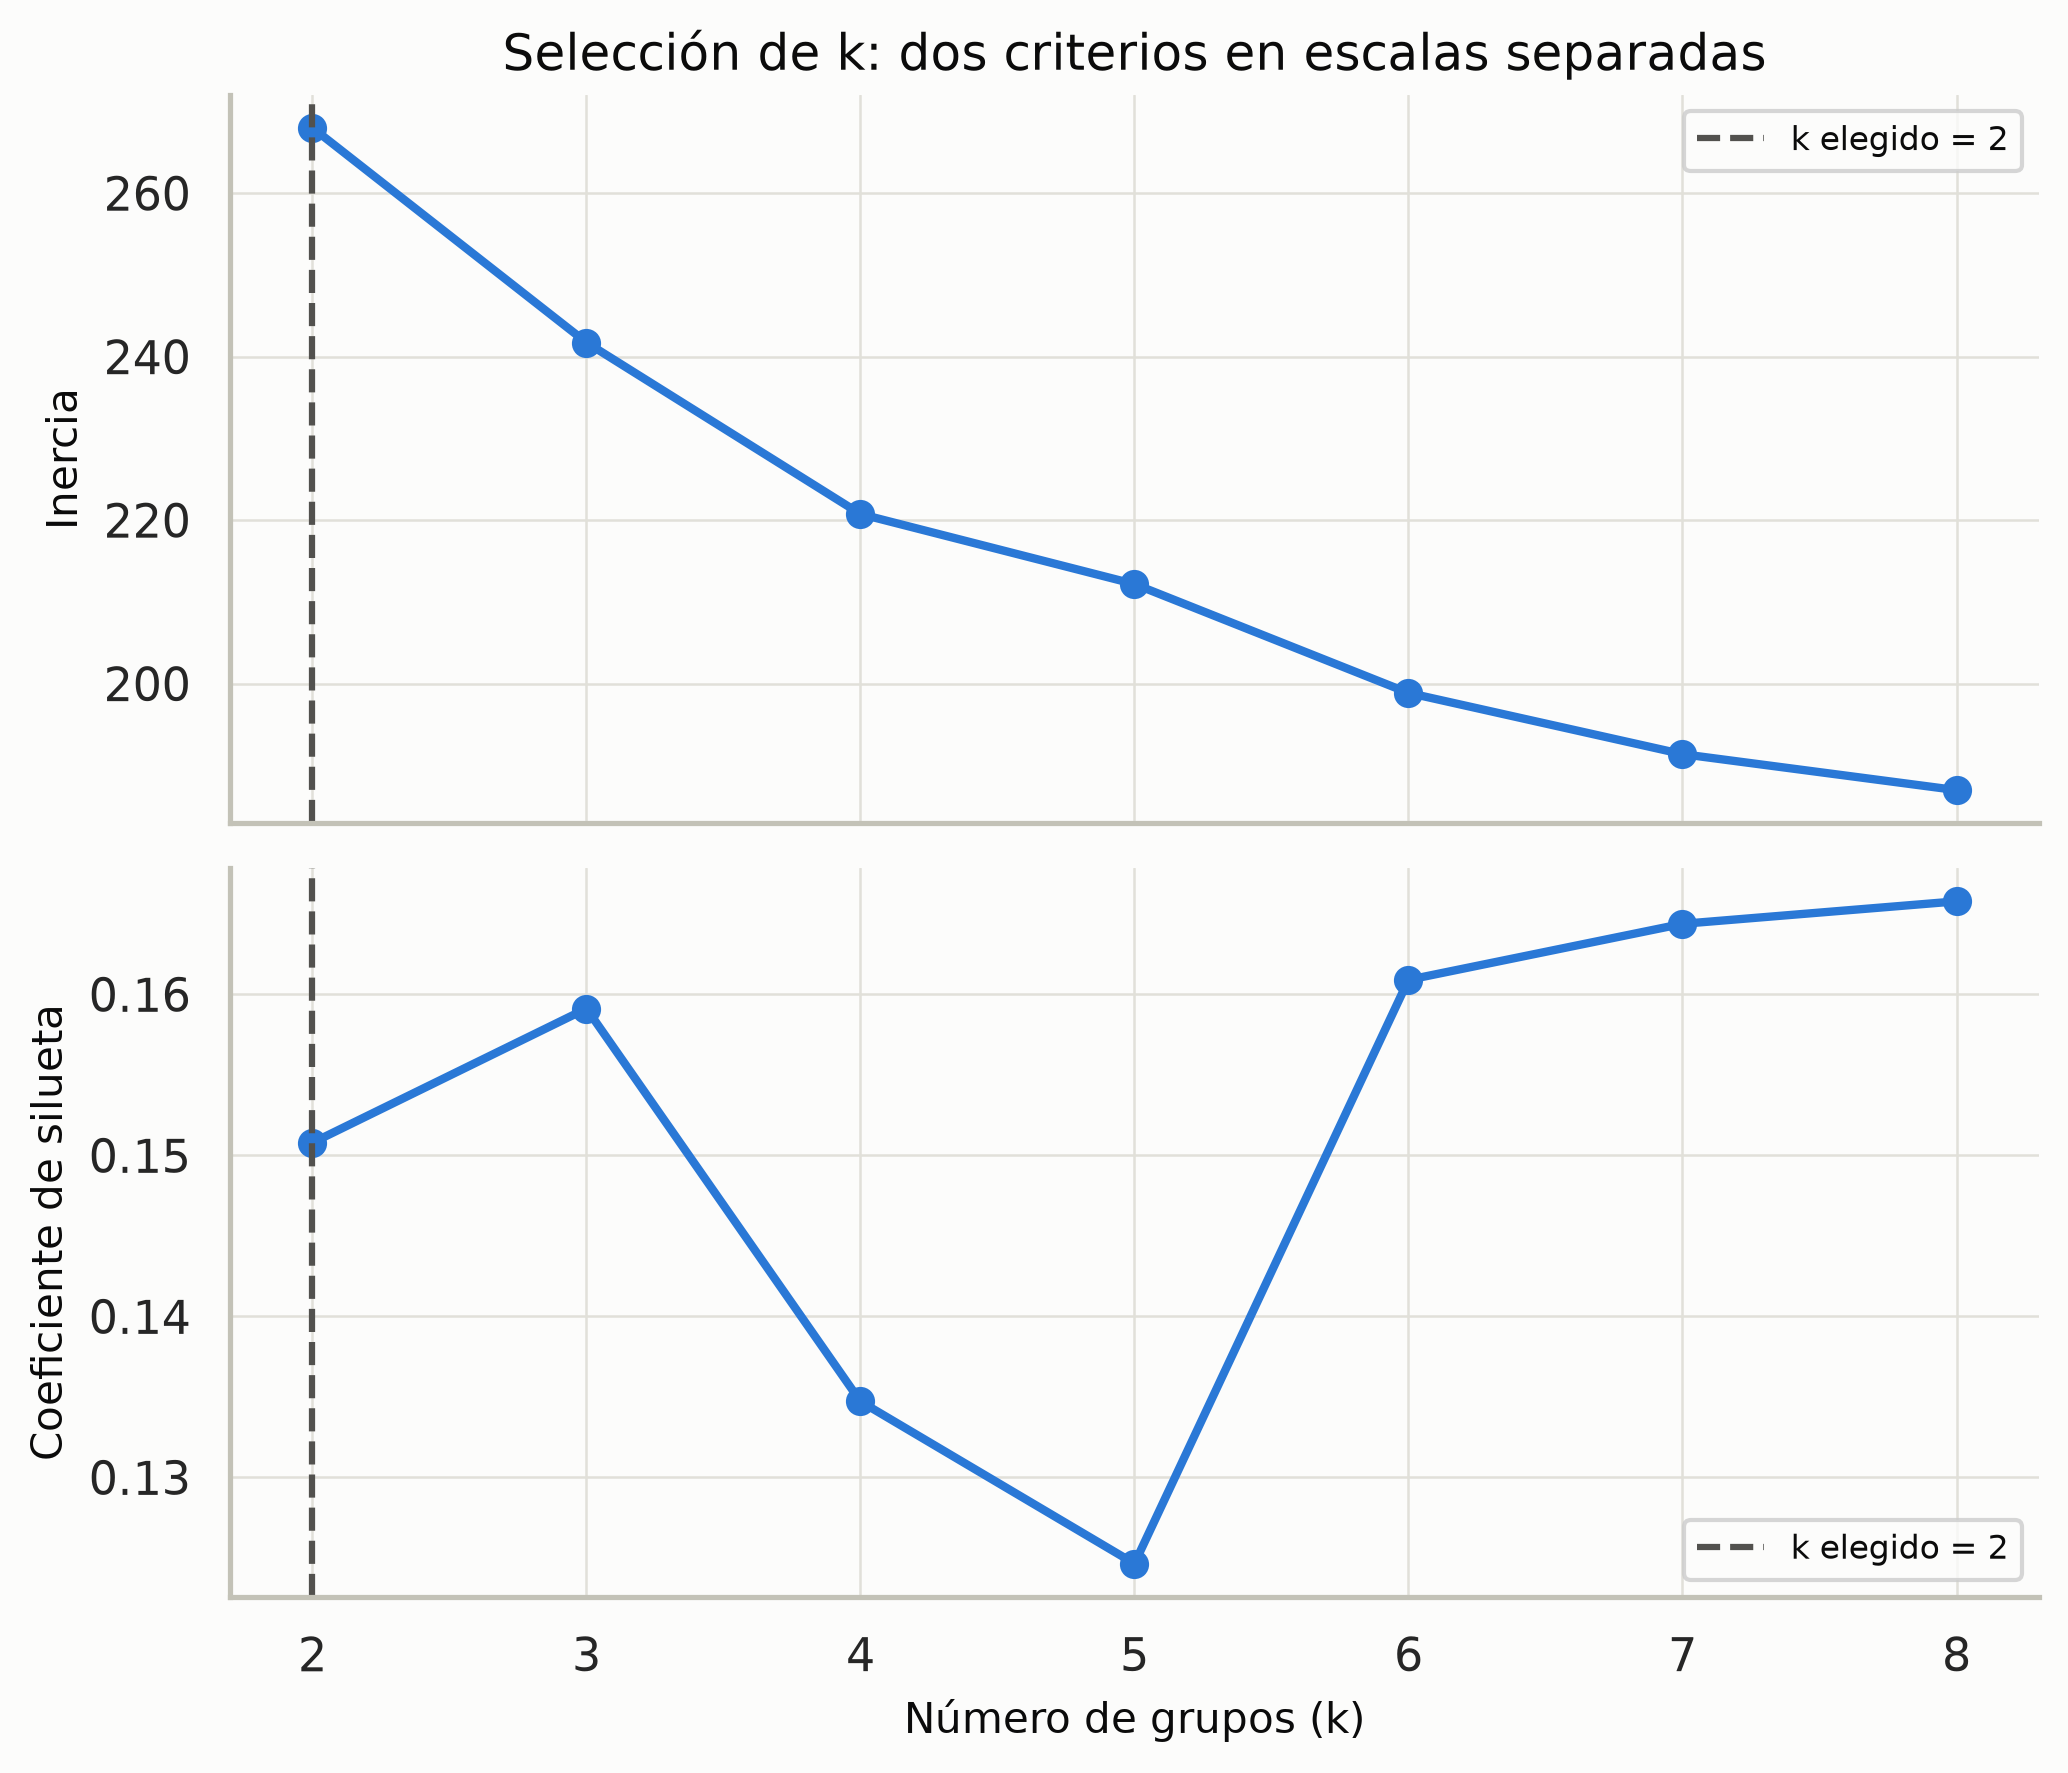
\includegraphics[width=0.86\textwidth]{img/08_seleccion_k.png}
\caption{Inercia y silueta para $k=2,\ldots,8$, en paneles con escalas independientes. La inercia disminuye al aumentar el número de grupos, pero no constituye por sí sola una mejora de interpretación.}
\label{fig:seleccion-k}
\end{figure}

La mejor silueta observada es 0,1658 con $k=8$. La regla predefinida elige el menor $k$ cuya silueta queda a menos de 0,02 del máximo: resulta \textbf{$k=2$}, con silueta 0,1508 e inercia 267,9952. La silueta es baja en todos los casos, por lo que la separación no es fuerte. La elección prioriza una descripción sencilla; no demuestra que existan exactamente dos familias musicales naturales.

El grupo 0 contiene 28 artistas y se caracteriza, por sobrerrepresentación respecto al conjunto, mediante \texttt{spanish hip-hop}, \texttt{rap} y \texttt{spanish rap}. El grupo 1 contiene 105 artistas y sus etiquetas de mayor sobrerrepresentación son \texttt{80s}, \texttt{alternative} y \texttt{alternative metal}; su mayor tamaño y heterogeneidad impiden resumirlo como un único género. Las etiquetas del perfil se eligen por cociente de prevalencias (\emph{lift}), no por frecuencia absoluta dentro del grupo.

\begin{table}[H]
\centering
\begin{tabular}{lrrr}
\hline
Grupo & Artistas únicos & Presentes en Jorge & Presentes en Pablo \\
\hline
0 & 28 & 5 & 24 \\
1 & 105 & 64 & 45 \\
\hline
\end{tabular}
\caption{Pertenencia de los artistas agrupados a los rankings de cada usuario. Un artista compartido cuenta en ambas columnas, por lo que estas no suman el total de artistas únicos.}
\label{tab:clusters-usuarios}
\end{table}

\begin{figure}[H]
\centering
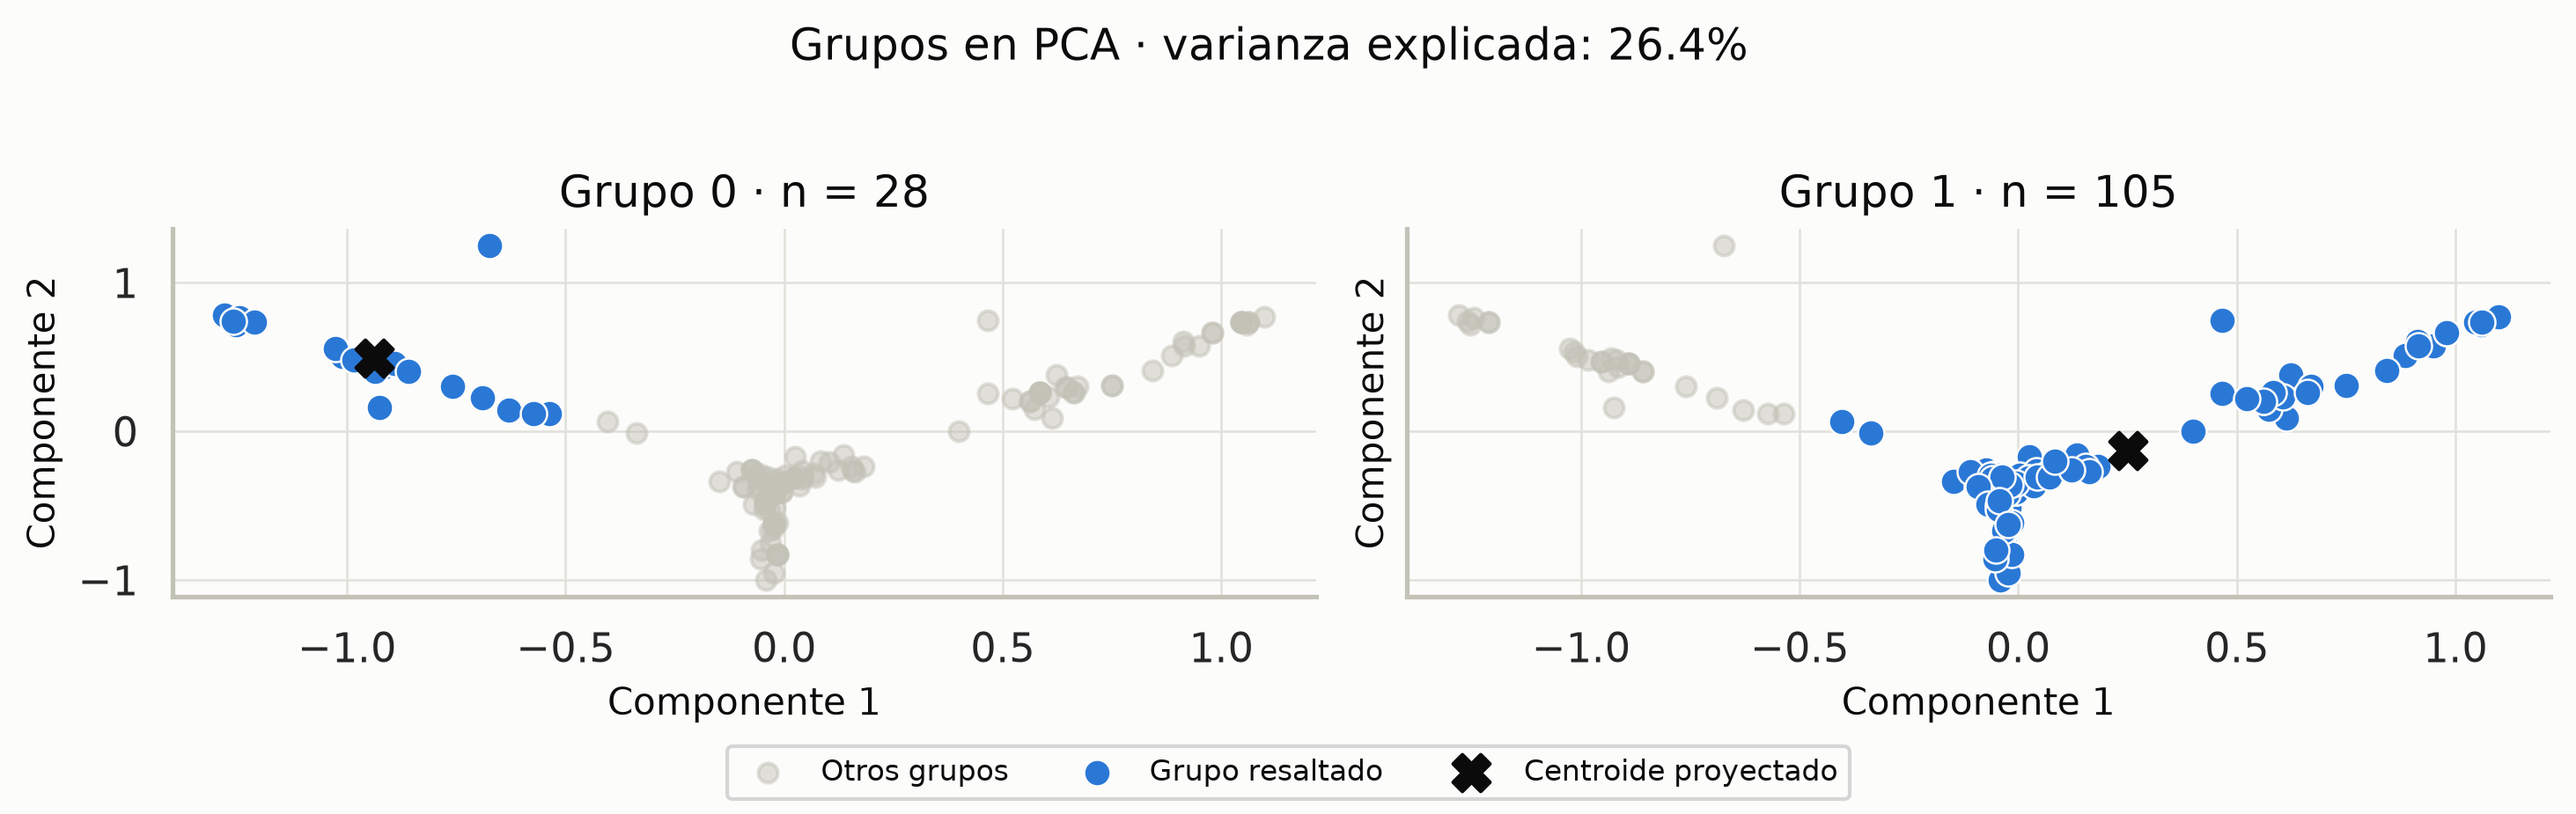
\includegraphics[width=\textwidth]{img/07_clustering_pca.png}
\caption{Proyección PCA con un panel por grupo. El azul destaca el grupo y el gris da contexto; la cruz representa su centroide proyectado. El ajuste de K-Means se realiza en las 52 dimensiones originales, no en este plano.}
\label{fig:pca}
\end{figure}

Las dos primeras componentes explican el \textbf{26,42\%} de la varianza. La proyección pierde casi tres cuartas partes de la variación: ni la proximidad ni la separación visual en dos dimensiones bastan para validar el agrupamiento. El grupo orientado al rap reúne una fracción mayor del perfil de Pablo (24 de sus 69 artistas agrupados) que del de Jorge (5 de 69), en consonancia con las frecuencias de etiquetas, sin constituir una prueba independiente de ellas.

\begin{figure}[H]
\centering
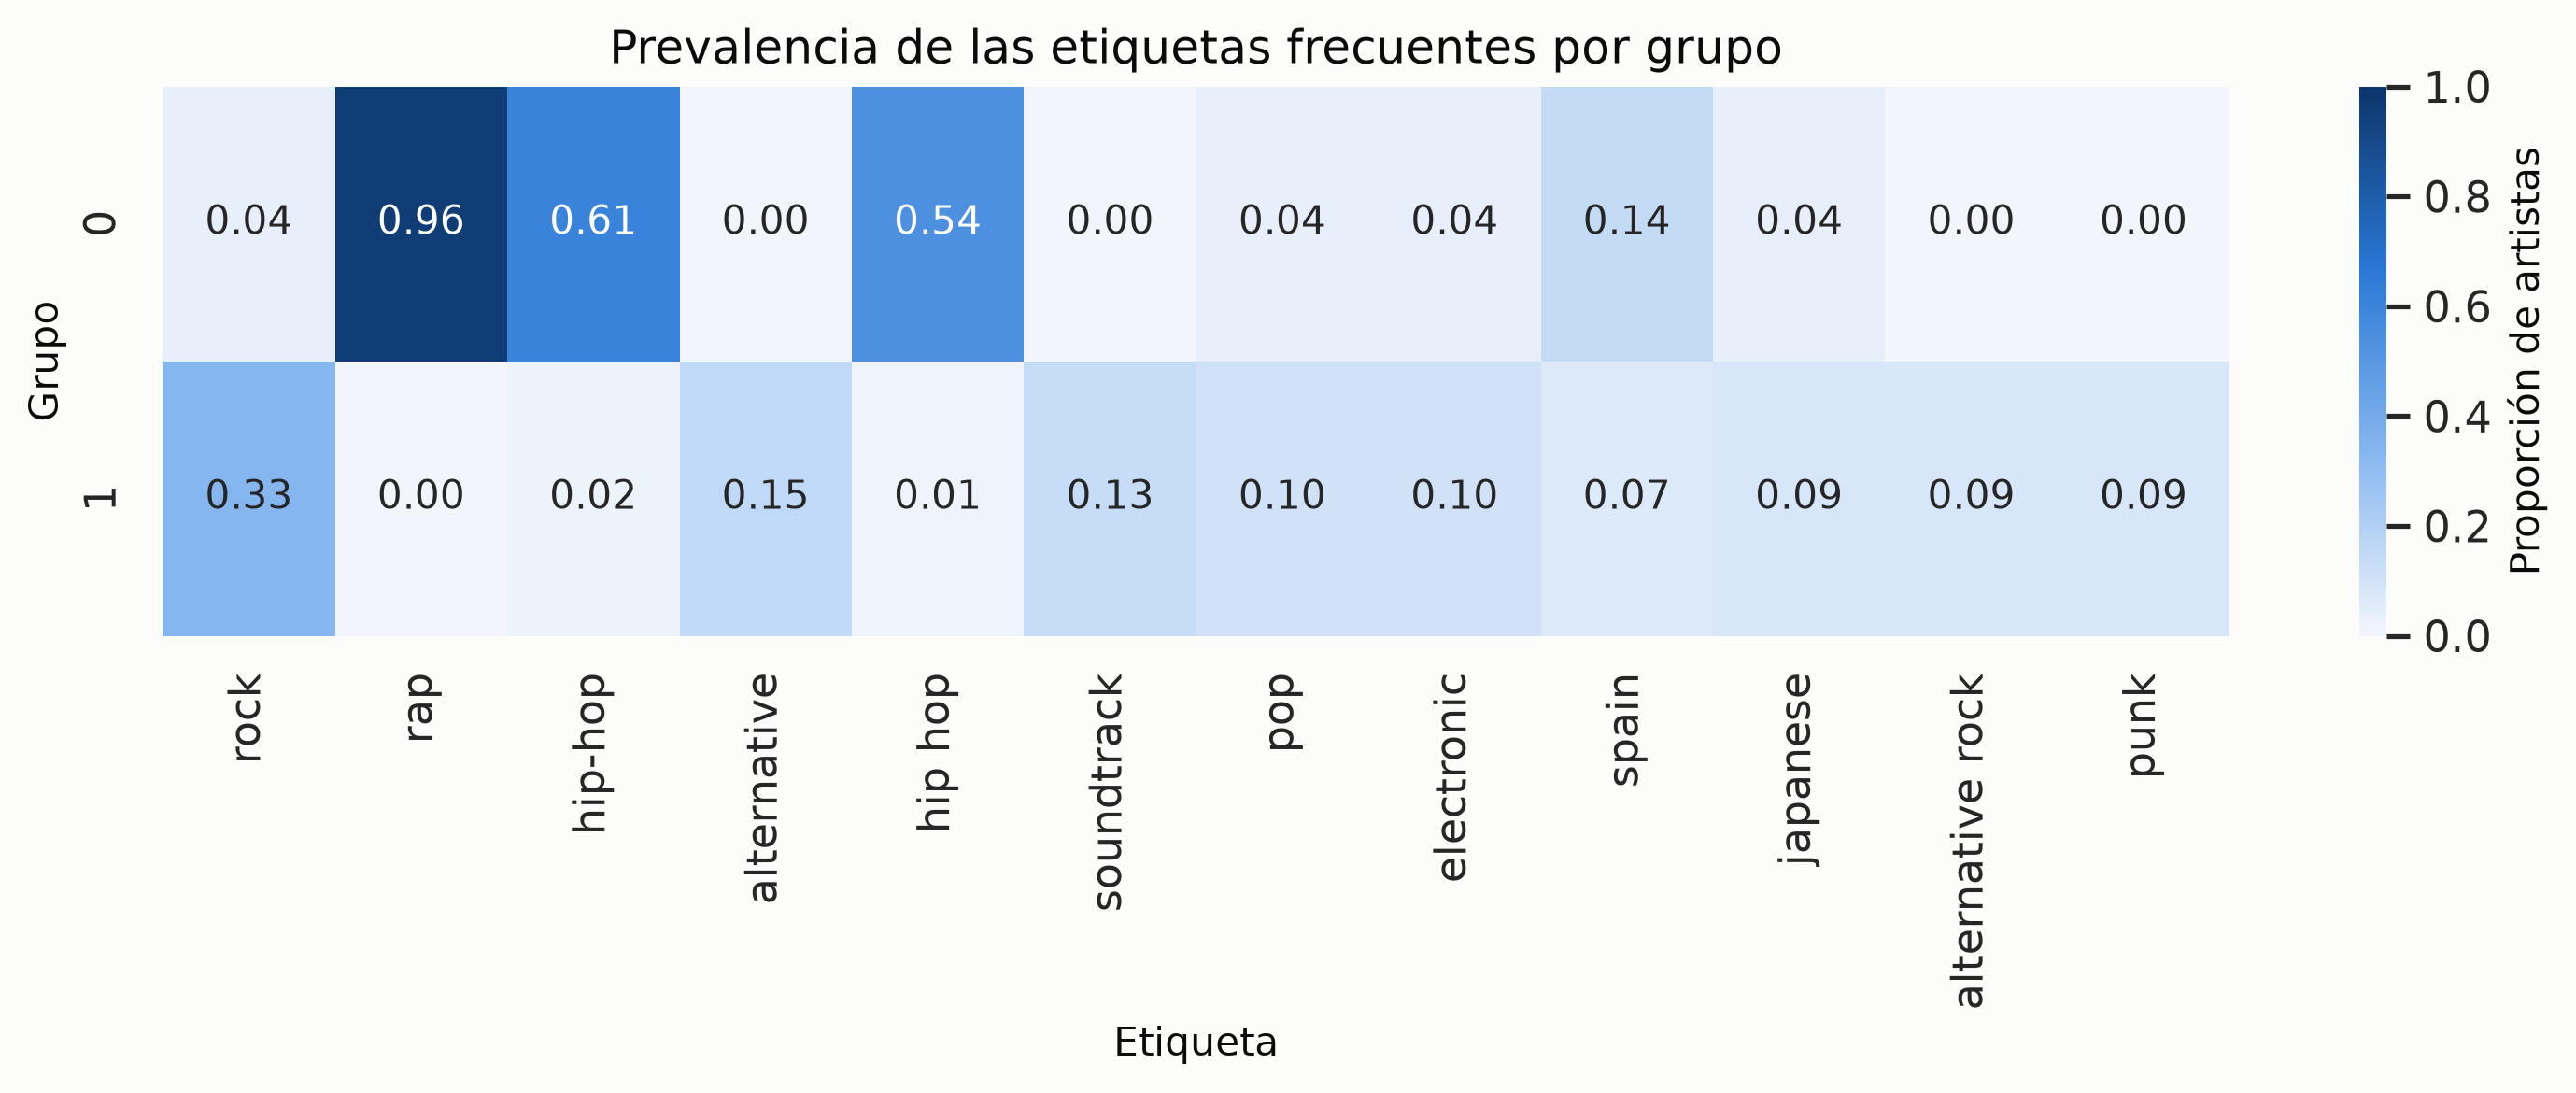
\includegraphics[width=\textwidth]{img/07b_perfil_clusters.png}
\caption{Prevalencia interna de las doce etiquetas más frecuentes de la matriz. La escala secuencial común representa proporciones entre 0 y 1; esta vista complementa las etiquetas elegidas por \emph{lift}.}
\label{fig:perfil-clusters}
\end{figure}

% ============================================
% ===== CAPÍTULO 6: CONCLUSIONES =====
% ============================================

\chapter*{Conclusiones}
\addcontentsline{toc}{chapter}{6. Conclusiones}
\label{chap:conclusiones}

\begin{tcolorbox}[colback=yellow!10, colframe=yellow!60!black, title=Pendiente de completar]
Las conclusiones definitivas se redactarán una vez completado el análisis y la visualización de resultados (Capítulos~\ref{chap:modelo} y~\ref{chap:resultados}). A continuación se dejan algunas conclusiones preliminares, centradas en el propio proceso de obtención de datos.
\end{tcolorbox}

\section{Conclusiones sobre el proceso de obtención de datos}
\label{sec:conclusiones-datos}

\begin{itemize}
    \item Combinar dos APIs externas (Spotify y Last.fm) permite enriquecer un conjunto de datos personal con información que ninguna de las dos fuentes ofrece de forma completa por sí sola, a costa de introducir ruido y huecos (artistas sin género) propios de combinar fuentes de distinta calidad y cobertura.
    \item El uso de una caché en memoria por artista único, en lugar de consultar Last.fm una vez por cada fila del conjunto de datos, resultó clave para mantener el proceso dentro de los límites de peticiones de la API externa.
    \item Trabajar con datos personales y dinámicos (dependientes del usuario autenticado y del momento de la consulta) implica que los resultados de este proyecto no son directamente reproducibles por un tercero sin sus propias credenciales y su propio historial de escucha, a diferencia de un conjunto de datos abierto y estático.
\end{itemize}

\section{Conclusiones del análisis}
\label{sec:conclusiones-analisis}

\textit{(Pendiente de redactar tras completar los Capítulos~\ref{chap:modelo} y~\ref{chap:resultados}: diversidad de géneros por usuario, estabilidad del gusto musical entre rangos temporales, grado de afinidad musical entre los dos autores y, en su caso, interpretación de los grupos obtenidos mediante \emph{clustering}.)}

\section{Limitaciones y trabajo futuro}
\label{sec:limitaciones}

\begin{itemize}
    \item El filtro de etiquetas no musicales de Last.fm (\texttt{IGNORAR}) es manual y no exhaustivo; podría mejorarse con una lista de géneros de referencia o un modelo de clasificación de etiquetas.
    \item El análisis se limita a dos usuarios; las conclusiones sobre similitud/diversidad musical no son generalizables más allá de los propios autores.
    \item La línea de afinidad usuario--artista (\S\ref{sec:recomendacion}) se apoya en similitud de contenido precisamente porque no existe una fuente fiable de ejemplos negativos (Spotify no expone artistas bloqueados/ocultados); un clasificador supervisado real de ``le gusta / no le gusta'' quedaría fuera del alcance de los datos disponibles.
    \item La \emph{Spotify Web API} ya no ofrece, para aplicaciones nuevas, los \emph{endpoints} de \texttt{audio-features} ni \texttt{related-artists} (restringidos desde noviembre de 2024), lo que limita el enriquecimiento a lo que puedan aportar fuentes externas como Last.fm, Deezer o MusicBrainz (\S\ref{sec:enriquecimiento}).
    \item Como ampliación, podría incorporarse también el historial de canciones más escuchadas (no solo artistas) además de los atributos de popularidad y similitud ya planteados.
\end{itemize}




\end{document}
